\documentclass[12pt]{article}
\usepackage[letterpaper, left=15mm, right=15mm, top=21mm, bottom=19mm, headheight=15pt, headsep=5mm, footskip=9mm]{geometry}
\usepackage[T1]{fontenc}
\usepackage{tgheros}
\renewcommand{\familydefault}{\sfdefault}
\usepackage{tikz}
\usepackage{fancyhdr}
\pagestyle{fancy}
\fancyhf{}
\lhead{Week 53 / Connecting networks / Grades 2--3}
\lfoot{\small Bellingham Math Circle / Week 53 / W53-RV-M-v1}
\rfoot{\small \thepage}
\renewcommand{\headrulewidth}{0.4pt}
\setlength{\parindent}{0pt}
\setlength{\parskip}{0pt}
\linespread{1.06}
\newcommand{\prob}[1]{\textbf{Problem #1:}}
\newcommand{\ans}[1]{\rule[-0.6ex]{#1}{0.5pt}}
\begin{document}

Buy a link by laying a marker along it and putting its price in counters in the tray. A network is a set of bought links that lets the pawn walk on markers between every two places.

\vspace{3mm}
\prob{1} Buy the cheapest network you can on this map. How many different networks cost exactly that much? Draw them.

\par\begin{center}
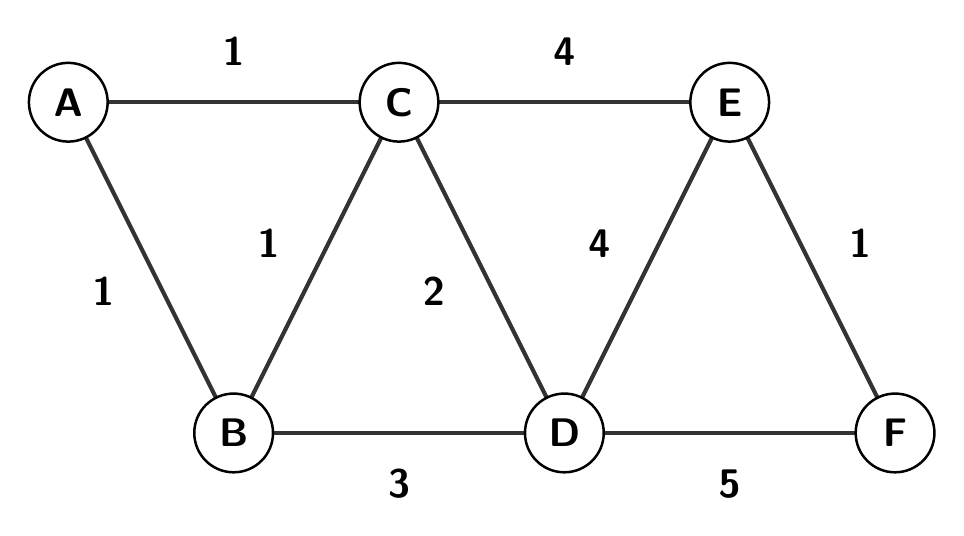
\begin{tikzpicture}[x=1mm,y=1mm]
\draw[line width=1.5pt, black!80] (5.00,51.46) -- (26.00,9.46);
\draw[line width=1.5pt, black!80] (5.00,51.46) -- (47.00,51.46);
\draw[line width=1.5pt, black!80] (26.00,9.46) -- (47.00,51.46);
\draw[line width=1.5pt, black!80] (47.00,51.46) -- (68.00,9.46);
\draw[line width=1.5pt, black!80] (26.00,9.46) -- (68.00,9.46);
\draw[line width=1.5pt, black!80] (47.00,51.46) -- (89.00,51.46);
\draw[line width=1.5pt, black!80] (68.00,9.46) -- (89.00,51.46);
\draw[line width=1.5pt, black!80] (89.00,51.46) -- (110.00,9.46);
\draw[line width=1.5pt, black!80] (68.00,9.46) -- (110.00,9.46);
\node[fill=white, inner sep=0, minimum width=4.40mm, minimum height=6.00mm, font=\Large\bfseries] at (9.44,27.44) {1};
\node[fill=white, inner sep=0, minimum width=4.40mm, minimum height=6.00mm, font=\Large\bfseries] at (26.00,57.93) {1};
\node[fill=white, inner sep=0, minimum width=4.40mm, minimum height=6.00mm, font=\Large\bfseries] at (30.44,33.49) {1};
\node[fill=white, inner sep=0, minimum width=4.40mm, minimum height=6.00mm, font=\Large\bfseries] at (51.44,27.44) {2};
\node[fill=white, inner sep=0, minimum width=4.40mm, minimum height=6.00mm, font=\Large\bfseries] at (47.00,3.00) {3};
\node[fill=white, inner sep=0, minimum width=4.40mm, minimum height=6.00mm, font=\Large\bfseries] at (68.00,57.93) {4};
\node[fill=white, inner sep=0, minimum width=4.40mm, minimum height=6.00mm, font=\Large\bfseries] at (72.44,33.49) {4};
\node[fill=white, inner sep=0, minimum width=4.40mm, minimum height=6.00mm, font=\Large\bfseries] at (105.56,33.49) {1};
\node[fill=white, inner sep=0, minimum width=4.40mm, minimum height=6.00mm, font=\Large\bfseries] at (89.00,3.00) {5};
\node[circle, draw, line width=0.9pt, fill=white, minimum size=10.00mm, inner sep=0, font=\Large\bfseries] at (5.00,51.46) {A};
\node[circle, draw, line width=0.9pt, fill=white, minimum size=10.00mm, inner sep=0, font=\Large\bfseries] at (47.00,51.46) {C};
\node[circle, draw, line width=0.9pt, fill=white, minimum size=10.00mm, inner sep=0, font=\Large\bfseries] at (89.00,51.46) {E};
\node[circle, draw, line width=0.9pt, fill=white, minimum size=10.00mm, inner sep=0, font=\Large\bfseries] at (26.00,9.46) {B};
\node[circle, draw, line width=0.9pt, fill=white, minimum size=10.00mm, inner sep=0, font=\Large\bfseries] at (68.00,9.46) {D};
\node[circle, draw, line width=0.9pt, fill=white, minimum size=10.00mm, inner sep=0, font=\Large\bfseries] at (110.00,9.46) {F};
\end{tikzpicture}
\end{center}\par

\vspace{-1mm}
\par\begin{center}
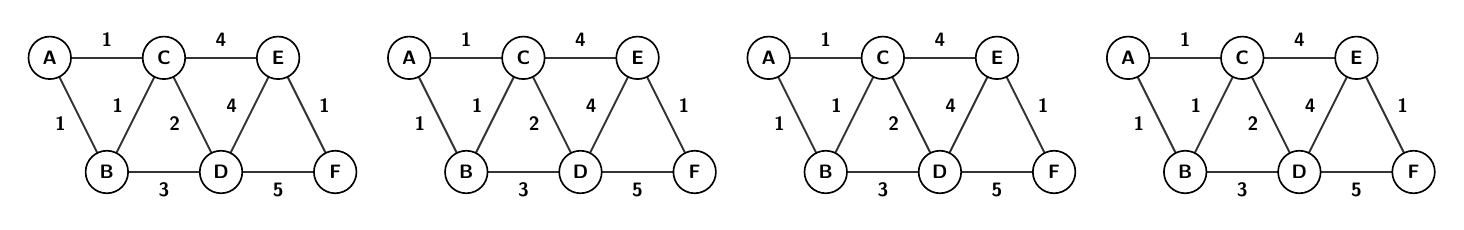
\begin{tikzpicture}[x=1mm,y=1mm]
\draw[line width=0.7pt, black!80] (2.70,18.32) -- (9.95,3.82);
\draw[line width=0.7pt, black!80] (2.70,18.32) -- (17.20,18.32);
\draw[line width=0.7pt, black!80] (9.95,3.82) -- (17.20,18.32);
\draw[line width=0.7pt, black!80] (17.20,18.32) -- (24.45,3.82);
\draw[line width=0.7pt, black!80] (9.95,3.82) -- (24.45,3.82);
\draw[line width=0.7pt, black!80] (17.20,18.32) -- (31.70,18.32);
\draw[line width=0.7pt, black!80] (24.45,3.82) -- (31.70,18.32);
\draw[line width=0.7pt, black!80] (31.70,18.32) -- (38.95,3.82);
\draw[line width=0.7pt, black!80] (24.45,3.82) -- (38.95,3.82);
\node[fill=white, inner sep=0, minimum width=2.30mm, minimum height=3.00mm, font=\scriptsize\bfseries] at (4.07,9.95) {1};
\node[fill=white, inner sep=0, minimum width=2.30mm, minimum height=3.00mm, font=\scriptsize\bfseries] at (9.95,20.65) {1};
\node[fill=white, inner sep=0, minimum width=2.30mm, minimum height=3.00mm, font=\scriptsize\bfseries] at (11.32,12.20) {1};
\node[fill=white, inner sep=0, minimum width=2.30mm, minimum height=3.00mm, font=\scriptsize\bfseries] at (18.57,9.95) {2};
\node[fill=white, inner sep=0, minimum width=2.30mm, minimum height=3.00mm, font=\scriptsize\bfseries] at (17.20,1.50) {3};
\node[fill=white, inner sep=0, minimum width=2.30mm, minimum height=3.00mm, font=\scriptsize\bfseries] at (24.45,20.65) {4};
\node[fill=white, inner sep=0, minimum width=2.30mm, minimum height=3.00mm, font=\scriptsize\bfseries] at (25.82,12.20) {4};
\node[fill=white, inner sep=0, minimum width=2.30mm, minimum height=3.00mm, font=\scriptsize\bfseries] at (37.58,12.20) {1};
\node[fill=white, inner sep=0, minimum width=2.30mm, minimum height=3.00mm, font=\scriptsize\bfseries] at (31.70,1.50) {5};
\node[circle, draw, line width=0.6pt, fill=white, minimum size=5.40mm, inner sep=0, font=\scriptsize\bfseries] at (2.70,18.32) {A};
\node[circle, draw, line width=0.6pt, fill=white, minimum size=5.40mm, inner sep=0, font=\scriptsize\bfseries] at (17.20,18.32) {C};
\node[circle, draw, line width=0.6pt, fill=white, minimum size=5.40mm, inner sep=0, font=\scriptsize\bfseries] at (31.70,18.32) {E};
\node[circle, draw, line width=0.6pt, fill=white, minimum size=5.40mm, inner sep=0, font=\scriptsize\bfseries] at (9.95,3.82) {B};
\node[circle, draw, line width=0.6pt, fill=white, minimum size=5.40mm, inner sep=0, font=\scriptsize\bfseries] at (24.45,3.82) {D};
\node[circle, draw, line width=0.6pt, fill=white, minimum size=5.40mm, inner sep=0, font=\scriptsize\bfseries] at (38.95,3.82) {F};
\draw[line width=0.7pt, black!80] (48.35,18.32) -- (55.60,3.82);
\draw[line width=0.7pt, black!80] (48.35,18.32) -- (62.85,18.32);
\draw[line width=0.7pt, black!80] (55.60,3.82) -- (62.85,18.32);
\draw[line width=0.7pt, black!80] (62.85,18.32) -- (70.10,3.82);
\draw[line width=0.7pt, black!80] (55.60,3.82) -- (70.10,3.82);
\draw[line width=0.7pt, black!80] (62.85,18.32) -- (77.35,18.32);
\draw[line width=0.7pt, black!80] (70.10,3.82) -- (77.35,18.32);
\draw[line width=0.7pt, black!80] (77.35,18.32) -- (84.60,3.82);
\draw[line width=0.7pt, black!80] (70.10,3.82) -- (84.60,3.82);
\node[fill=white, inner sep=0, minimum width=2.30mm, minimum height=3.00mm, font=\scriptsize\bfseries] at (49.72,9.95) {1};
\node[fill=white, inner sep=0, minimum width=2.30mm, minimum height=3.00mm, font=\scriptsize\bfseries] at (55.60,20.65) {1};
\node[fill=white, inner sep=0, minimum width=2.30mm, minimum height=3.00mm, font=\scriptsize\bfseries] at (56.97,12.20) {1};
\node[fill=white, inner sep=0, minimum width=2.30mm, minimum height=3.00mm, font=\scriptsize\bfseries] at (64.22,9.95) {2};
\node[fill=white, inner sep=0, minimum width=2.30mm, minimum height=3.00mm, font=\scriptsize\bfseries] at (62.85,1.50) {3};
\node[fill=white, inner sep=0, minimum width=2.30mm, minimum height=3.00mm, font=\scriptsize\bfseries] at (70.10,20.65) {4};
\node[fill=white, inner sep=0, minimum width=2.30mm, minimum height=3.00mm, font=\scriptsize\bfseries] at (71.47,12.20) {4};
\node[fill=white, inner sep=0, minimum width=2.30mm, minimum height=3.00mm, font=\scriptsize\bfseries] at (83.23,12.20) {1};
\node[fill=white, inner sep=0, minimum width=2.30mm, minimum height=3.00mm, font=\scriptsize\bfseries] at (77.35,1.50) {5};
\node[circle, draw, line width=0.6pt, fill=white, minimum size=5.40mm, inner sep=0, font=\scriptsize\bfseries] at (48.35,18.32) {A};
\node[circle, draw, line width=0.6pt, fill=white, minimum size=5.40mm, inner sep=0, font=\scriptsize\bfseries] at (62.85,18.32) {C};
\node[circle, draw, line width=0.6pt, fill=white, minimum size=5.40mm, inner sep=0, font=\scriptsize\bfseries] at (77.35,18.32) {E};
\node[circle, draw, line width=0.6pt, fill=white, minimum size=5.40mm, inner sep=0, font=\scriptsize\bfseries] at (55.60,3.82) {B};
\node[circle, draw, line width=0.6pt, fill=white, minimum size=5.40mm, inner sep=0, font=\scriptsize\bfseries] at (70.10,3.82) {D};
\node[circle, draw, line width=0.6pt, fill=white, minimum size=5.40mm, inner sep=0, font=\scriptsize\bfseries] at (84.60,3.82) {F};
\draw[line width=0.7pt, black!80] (94.00,18.32) -- (101.25,3.82);
\draw[line width=0.7pt, black!80] (94.00,18.32) -- (108.50,18.32);
\draw[line width=0.7pt, black!80] (101.25,3.82) -- (108.50,18.32);
\draw[line width=0.7pt, black!80] (108.50,18.32) -- (115.75,3.82);
\draw[line width=0.7pt, black!80] (101.25,3.82) -- (115.75,3.82);
\draw[line width=0.7pt, black!80] (108.50,18.32) -- (123.00,18.32);
\draw[line width=0.7pt, black!80] (115.75,3.82) -- (123.00,18.32);
\draw[line width=0.7pt, black!80] (123.00,18.32) -- (130.25,3.82);
\draw[line width=0.7pt, black!80] (115.75,3.82) -- (130.25,3.82);
\node[fill=white, inner sep=0, minimum width=2.30mm, minimum height=3.00mm, font=\scriptsize\bfseries] at (95.37,9.95) {1};
\node[fill=white, inner sep=0, minimum width=2.30mm, minimum height=3.00mm, font=\scriptsize\bfseries] at (101.25,20.65) {1};
\node[fill=white, inner sep=0, minimum width=2.30mm, minimum height=3.00mm, font=\scriptsize\bfseries] at (102.62,12.20) {1};
\node[fill=white, inner sep=0, minimum width=2.30mm, minimum height=3.00mm, font=\scriptsize\bfseries] at (109.87,9.95) {2};
\node[fill=white, inner sep=0, minimum width=2.30mm, minimum height=3.00mm, font=\scriptsize\bfseries] at (108.50,1.50) {3};
\node[fill=white, inner sep=0, minimum width=2.30mm, minimum height=3.00mm, font=\scriptsize\bfseries] at (115.75,20.65) {4};
\node[fill=white, inner sep=0, minimum width=2.30mm, minimum height=3.00mm, font=\scriptsize\bfseries] at (117.12,12.20) {4};
\node[fill=white, inner sep=0, minimum width=2.30mm, minimum height=3.00mm, font=\scriptsize\bfseries] at (128.88,12.20) {1};
\node[fill=white, inner sep=0, minimum width=2.30mm, minimum height=3.00mm, font=\scriptsize\bfseries] at (123.00,1.50) {5};
\node[circle, draw, line width=0.6pt, fill=white, minimum size=5.40mm, inner sep=0, font=\scriptsize\bfseries] at (94.00,18.32) {A};
\node[circle, draw, line width=0.6pt, fill=white, minimum size=5.40mm, inner sep=0, font=\scriptsize\bfseries] at (108.50,18.32) {C};
\node[circle, draw, line width=0.6pt, fill=white, minimum size=5.40mm, inner sep=0, font=\scriptsize\bfseries] at (123.00,18.32) {E};
\node[circle, draw, line width=0.6pt, fill=white, minimum size=5.40mm, inner sep=0, font=\scriptsize\bfseries] at (101.25,3.82) {B};
\node[circle, draw, line width=0.6pt, fill=white, minimum size=5.40mm, inner sep=0, font=\scriptsize\bfseries] at (115.75,3.82) {D};
\node[circle, draw, line width=0.6pt, fill=white, minimum size=5.40mm, inner sep=0, font=\scriptsize\bfseries] at (130.25,3.82) {F};
\draw[line width=0.7pt, black!80] (139.65,18.32) -- (146.90,3.82);
\draw[line width=0.7pt, black!80] (139.65,18.32) -- (154.15,18.32);
\draw[line width=0.7pt, black!80] (146.90,3.82) -- (154.15,18.32);
\draw[line width=0.7pt, black!80] (154.15,18.32) -- (161.40,3.82);
\draw[line width=0.7pt, black!80] (146.90,3.82) -- (161.40,3.82);
\draw[line width=0.7pt, black!80] (154.15,18.32) -- (168.65,18.32);
\draw[line width=0.7pt, black!80] (161.40,3.82) -- (168.65,18.32);
\draw[line width=0.7pt, black!80] (168.65,18.32) -- (175.90,3.82);
\draw[line width=0.7pt, black!80] (161.40,3.82) -- (175.90,3.82);
\node[fill=white, inner sep=0, minimum width=2.30mm, minimum height=3.00mm, font=\scriptsize\bfseries] at (141.02,9.95) {1};
\node[fill=white, inner sep=0, minimum width=2.30mm, minimum height=3.00mm, font=\scriptsize\bfseries] at (146.90,20.65) {1};
\node[fill=white, inner sep=0, minimum width=2.30mm, minimum height=3.00mm, font=\scriptsize\bfseries] at (148.27,12.20) {1};
\node[fill=white, inner sep=0, minimum width=2.30mm, minimum height=3.00mm, font=\scriptsize\bfseries] at (155.52,9.95) {2};
\node[fill=white, inner sep=0, minimum width=2.30mm, minimum height=3.00mm, font=\scriptsize\bfseries] at (154.15,1.50) {3};
\node[fill=white, inner sep=0, minimum width=2.30mm, minimum height=3.00mm, font=\scriptsize\bfseries] at (161.40,20.65) {4};
\node[fill=white, inner sep=0, minimum width=2.30mm, minimum height=3.00mm, font=\scriptsize\bfseries] at (162.77,12.20) {4};
\node[fill=white, inner sep=0, minimum width=2.30mm, minimum height=3.00mm, font=\scriptsize\bfseries] at (174.53,12.20) {1};
\node[fill=white, inner sep=0, minimum width=2.30mm, minimum height=3.00mm, font=\scriptsize\bfseries] at (168.65,1.50) {5};
\node[circle, draw, line width=0.6pt, fill=white, minimum size=5.40mm, inner sep=0, font=\scriptsize\bfseries] at (139.65,18.32) {A};
\node[circle, draw, line width=0.6pt, fill=white, minimum size=5.40mm, inner sep=0, font=\scriptsize\bfseries] at (154.15,18.32) {C};
\node[circle, draw, line width=0.6pt, fill=white, minimum size=5.40mm, inner sep=0, font=\scriptsize\bfseries] at (168.65,18.32) {E};
\node[circle, draw, line width=0.6pt, fill=white, minimum size=5.40mm, inner sep=0, font=\scriptsize\bfseries] at (146.90,3.82) {B};
\node[circle, draw, line width=0.6pt, fill=white, minimum size=5.40mm, inner sep=0, font=\scriptsize\bfseries] at (161.40,3.82) {D};
\node[circle, draw, line width=0.6pt, fill=white, minimum size=5.40mm, inner sep=0, font=\scriptsize\bfseries] at (175.90,3.82) {F};
\end{tikzpicture}
\end{center}\par

\vspace{-1mm}
\par\begin{center}
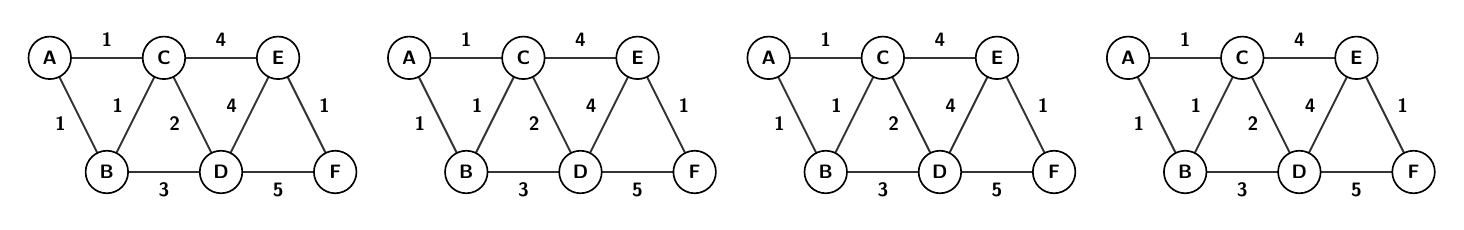
\begin{tikzpicture}[x=1mm,y=1mm]
\draw[line width=0.7pt, black!80] (2.70,18.32) -- (9.95,3.82);
\draw[line width=0.7pt, black!80] (2.70,18.32) -- (17.20,18.32);
\draw[line width=0.7pt, black!80] (9.95,3.82) -- (17.20,18.32);
\draw[line width=0.7pt, black!80] (17.20,18.32) -- (24.45,3.82);
\draw[line width=0.7pt, black!80] (9.95,3.82) -- (24.45,3.82);
\draw[line width=0.7pt, black!80] (17.20,18.32) -- (31.70,18.32);
\draw[line width=0.7pt, black!80] (24.45,3.82) -- (31.70,18.32);
\draw[line width=0.7pt, black!80] (31.70,18.32) -- (38.95,3.82);
\draw[line width=0.7pt, black!80] (24.45,3.82) -- (38.95,3.82);
\node[fill=white, inner sep=0, minimum width=2.30mm, minimum height=3.00mm, font=\scriptsize\bfseries] at (4.07,9.95) {1};
\node[fill=white, inner sep=0, minimum width=2.30mm, minimum height=3.00mm, font=\scriptsize\bfseries] at (9.95,20.65) {1};
\node[fill=white, inner sep=0, minimum width=2.30mm, minimum height=3.00mm, font=\scriptsize\bfseries] at (11.32,12.20) {1};
\node[fill=white, inner sep=0, minimum width=2.30mm, minimum height=3.00mm, font=\scriptsize\bfseries] at (18.57,9.95) {2};
\node[fill=white, inner sep=0, minimum width=2.30mm, minimum height=3.00mm, font=\scriptsize\bfseries] at (17.20,1.50) {3};
\node[fill=white, inner sep=0, minimum width=2.30mm, minimum height=3.00mm, font=\scriptsize\bfseries] at (24.45,20.65) {4};
\node[fill=white, inner sep=0, minimum width=2.30mm, minimum height=3.00mm, font=\scriptsize\bfseries] at (25.82,12.20) {4};
\node[fill=white, inner sep=0, minimum width=2.30mm, minimum height=3.00mm, font=\scriptsize\bfseries] at (37.58,12.20) {1};
\node[fill=white, inner sep=0, minimum width=2.30mm, minimum height=3.00mm, font=\scriptsize\bfseries] at (31.70,1.50) {5};
\node[circle, draw, line width=0.6pt, fill=white, minimum size=5.40mm, inner sep=0, font=\scriptsize\bfseries] at (2.70,18.32) {A};
\node[circle, draw, line width=0.6pt, fill=white, minimum size=5.40mm, inner sep=0, font=\scriptsize\bfseries] at (17.20,18.32) {C};
\node[circle, draw, line width=0.6pt, fill=white, minimum size=5.40mm, inner sep=0, font=\scriptsize\bfseries] at (31.70,18.32) {E};
\node[circle, draw, line width=0.6pt, fill=white, minimum size=5.40mm, inner sep=0, font=\scriptsize\bfseries] at (9.95,3.82) {B};
\node[circle, draw, line width=0.6pt, fill=white, minimum size=5.40mm, inner sep=0, font=\scriptsize\bfseries] at (24.45,3.82) {D};
\node[circle, draw, line width=0.6pt, fill=white, minimum size=5.40mm, inner sep=0, font=\scriptsize\bfseries] at (38.95,3.82) {F};
\draw[line width=0.7pt, black!80] (48.35,18.32) -- (55.60,3.82);
\draw[line width=0.7pt, black!80] (48.35,18.32) -- (62.85,18.32);
\draw[line width=0.7pt, black!80] (55.60,3.82) -- (62.85,18.32);
\draw[line width=0.7pt, black!80] (62.85,18.32) -- (70.10,3.82);
\draw[line width=0.7pt, black!80] (55.60,3.82) -- (70.10,3.82);
\draw[line width=0.7pt, black!80] (62.85,18.32) -- (77.35,18.32);
\draw[line width=0.7pt, black!80] (70.10,3.82) -- (77.35,18.32);
\draw[line width=0.7pt, black!80] (77.35,18.32) -- (84.60,3.82);
\draw[line width=0.7pt, black!80] (70.10,3.82) -- (84.60,3.82);
\node[fill=white, inner sep=0, minimum width=2.30mm, minimum height=3.00mm, font=\scriptsize\bfseries] at (49.72,9.95) {1};
\node[fill=white, inner sep=0, minimum width=2.30mm, minimum height=3.00mm, font=\scriptsize\bfseries] at (55.60,20.65) {1};
\node[fill=white, inner sep=0, minimum width=2.30mm, minimum height=3.00mm, font=\scriptsize\bfseries] at (56.97,12.20) {1};
\node[fill=white, inner sep=0, minimum width=2.30mm, minimum height=3.00mm, font=\scriptsize\bfseries] at (64.22,9.95) {2};
\node[fill=white, inner sep=0, minimum width=2.30mm, minimum height=3.00mm, font=\scriptsize\bfseries] at (62.85,1.50) {3};
\node[fill=white, inner sep=0, minimum width=2.30mm, minimum height=3.00mm, font=\scriptsize\bfseries] at (70.10,20.65) {4};
\node[fill=white, inner sep=0, minimum width=2.30mm, minimum height=3.00mm, font=\scriptsize\bfseries] at (71.47,12.20) {4};
\node[fill=white, inner sep=0, minimum width=2.30mm, minimum height=3.00mm, font=\scriptsize\bfseries] at (83.23,12.20) {1};
\node[fill=white, inner sep=0, minimum width=2.30mm, minimum height=3.00mm, font=\scriptsize\bfseries] at (77.35,1.50) {5};
\node[circle, draw, line width=0.6pt, fill=white, minimum size=5.40mm, inner sep=0, font=\scriptsize\bfseries] at (48.35,18.32) {A};
\node[circle, draw, line width=0.6pt, fill=white, minimum size=5.40mm, inner sep=0, font=\scriptsize\bfseries] at (62.85,18.32) {C};
\node[circle, draw, line width=0.6pt, fill=white, minimum size=5.40mm, inner sep=0, font=\scriptsize\bfseries] at (77.35,18.32) {E};
\node[circle, draw, line width=0.6pt, fill=white, minimum size=5.40mm, inner sep=0, font=\scriptsize\bfseries] at (55.60,3.82) {B};
\node[circle, draw, line width=0.6pt, fill=white, minimum size=5.40mm, inner sep=0, font=\scriptsize\bfseries] at (70.10,3.82) {D};
\node[circle, draw, line width=0.6pt, fill=white, minimum size=5.40mm, inner sep=0, font=\scriptsize\bfseries] at (84.60,3.82) {F};
\draw[line width=0.7pt, black!80] (94.00,18.32) -- (101.25,3.82);
\draw[line width=0.7pt, black!80] (94.00,18.32) -- (108.50,18.32);
\draw[line width=0.7pt, black!80] (101.25,3.82) -- (108.50,18.32);
\draw[line width=0.7pt, black!80] (108.50,18.32) -- (115.75,3.82);
\draw[line width=0.7pt, black!80] (101.25,3.82) -- (115.75,3.82);
\draw[line width=0.7pt, black!80] (108.50,18.32) -- (123.00,18.32);
\draw[line width=0.7pt, black!80] (115.75,3.82) -- (123.00,18.32);
\draw[line width=0.7pt, black!80] (123.00,18.32) -- (130.25,3.82);
\draw[line width=0.7pt, black!80] (115.75,3.82) -- (130.25,3.82);
\node[fill=white, inner sep=0, minimum width=2.30mm, minimum height=3.00mm, font=\scriptsize\bfseries] at (95.37,9.95) {1};
\node[fill=white, inner sep=0, minimum width=2.30mm, minimum height=3.00mm, font=\scriptsize\bfseries] at (101.25,20.65) {1};
\node[fill=white, inner sep=0, minimum width=2.30mm, minimum height=3.00mm, font=\scriptsize\bfseries] at (102.62,12.20) {1};
\node[fill=white, inner sep=0, minimum width=2.30mm, minimum height=3.00mm, font=\scriptsize\bfseries] at (109.87,9.95) {2};
\node[fill=white, inner sep=0, minimum width=2.30mm, minimum height=3.00mm, font=\scriptsize\bfseries] at (108.50,1.50) {3};
\node[fill=white, inner sep=0, minimum width=2.30mm, minimum height=3.00mm, font=\scriptsize\bfseries] at (115.75,20.65) {4};
\node[fill=white, inner sep=0, minimum width=2.30mm, minimum height=3.00mm, font=\scriptsize\bfseries] at (117.12,12.20) {4};
\node[fill=white, inner sep=0, minimum width=2.30mm, minimum height=3.00mm, font=\scriptsize\bfseries] at (128.88,12.20) {1};
\node[fill=white, inner sep=0, minimum width=2.30mm, minimum height=3.00mm, font=\scriptsize\bfseries] at (123.00,1.50) {5};
\node[circle, draw, line width=0.6pt, fill=white, minimum size=5.40mm, inner sep=0, font=\scriptsize\bfseries] at (94.00,18.32) {A};
\node[circle, draw, line width=0.6pt, fill=white, minimum size=5.40mm, inner sep=0, font=\scriptsize\bfseries] at (108.50,18.32) {C};
\node[circle, draw, line width=0.6pt, fill=white, minimum size=5.40mm, inner sep=0, font=\scriptsize\bfseries] at (123.00,18.32) {E};
\node[circle, draw, line width=0.6pt, fill=white, minimum size=5.40mm, inner sep=0, font=\scriptsize\bfseries] at (101.25,3.82) {B};
\node[circle, draw, line width=0.6pt, fill=white, minimum size=5.40mm, inner sep=0, font=\scriptsize\bfseries] at (115.75,3.82) {D};
\node[circle, draw, line width=0.6pt, fill=white, minimum size=5.40mm, inner sep=0, font=\scriptsize\bfseries] at (130.25,3.82) {F};
\draw[line width=0.7pt, black!80] (139.65,18.32) -- (146.90,3.82);
\draw[line width=0.7pt, black!80] (139.65,18.32) -- (154.15,18.32);
\draw[line width=0.7pt, black!80] (146.90,3.82) -- (154.15,18.32);
\draw[line width=0.7pt, black!80] (154.15,18.32) -- (161.40,3.82);
\draw[line width=0.7pt, black!80] (146.90,3.82) -- (161.40,3.82);
\draw[line width=0.7pt, black!80] (154.15,18.32) -- (168.65,18.32);
\draw[line width=0.7pt, black!80] (161.40,3.82) -- (168.65,18.32);
\draw[line width=0.7pt, black!80] (168.65,18.32) -- (175.90,3.82);
\draw[line width=0.7pt, black!80] (161.40,3.82) -- (175.90,3.82);
\node[fill=white, inner sep=0, minimum width=2.30mm, minimum height=3.00mm, font=\scriptsize\bfseries] at (141.02,9.95) {1};
\node[fill=white, inner sep=0, minimum width=2.30mm, minimum height=3.00mm, font=\scriptsize\bfseries] at (146.90,20.65) {1};
\node[fill=white, inner sep=0, minimum width=2.30mm, minimum height=3.00mm, font=\scriptsize\bfseries] at (148.27,12.20) {1};
\node[fill=white, inner sep=0, minimum width=2.30mm, minimum height=3.00mm, font=\scriptsize\bfseries] at (155.52,9.95) {2};
\node[fill=white, inner sep=0, minimum width=2.30mm, minimum height=3.00mm, font=\scriptsize\bfseries] at (154.15,1.50) {3};
\node[fill=white, inner sep=0, minimum width=2.30mm, minimum height=3.00mm, font=\scriptsize\bfseries] at (161.40,20.65) {4};
\node[fill=white, inner sep=0, minimum width=2.30mm, minimum height=3.00mm, font=\scriptsize\bfseries] at (162.77,12.20) {4};
\node[fill=white, inner sep=0, minimum width=2.30mm, minimum height=3.00mm, font=\scriptsize\bfseries] at (174.53,12.20) {1};
\node[fill=white, inner sep=0, minimum width=2.30mm, minimum height=3.00mm, font=\scriptsize\bfseries] at (168.65,1.50) {5};
\node[circle, draw, line width=0.6pt, fill=white, minimum size=5.40mm, inner sep=0, font=\scriptsize\bfseries] at (139.65,18.32) {A};
\node[circle, draw, line width=0.6pt, fill=white, minimum size=5.40mm, inner sep=0, font=\scriptsize\bfseries] at (154.15,18.32) {C};
\node[circle, draw, line width=0.6pt, fill=white, minimum size=5.40mm, inner sep=0, font=\scriptsize\bfseries] at (168.65,18.32) {E};
\node[circle, draw, line width=0.6pt, fill=white, minimum size=5.40mm, inner sep=0, font=\scriptsize\bfseries] at (146.90,3.82) {B};
\node[circle, draw, line width=0.6pt, fill=white, minimum size=5.40mm, inner sep=0, font=\scriptsize\bfseries] at (161.40,3.82) {D};
\node[circle, draw, line width=0.6pt, fill=white, minimum size=5.40mm, inner sep=0, font=\scriptsize\bfseries] at (175.90,3.82) {F};
\end{tikzpicture}
\end{center}\par

\vspace{1mm}
\prob{2} A route is a way for the pawn to walk from one place to another along links, such as ABD. Find a route from A to D whose biggest price is as small as possible. Do the same from B to D, from D to F and from A to F.

\vspace{4mm}
\begin{tabular}{@{}l@{\hspace{3mm}}l@{\hspace{8mm}}l@{}}
A to D: & route \ans{35mm} & biggest price \ans{14mm}\\[6mm]
B to D: & route \ans{35mm} & biggest price \ans{14mm}\\[6mm]
D to F: & route \ans{35mm} & biggest price \ans{14mm}\\[6mm]
A to F: & route \ans{35mm} & biggest price \ans{14mm}
\end{tabular}
\newpage

\prob{3} On the big map, lay markers on the links priced 1, and draw a ring around each group of places that the pawn can walk between on markers, as in the small pictures. Then add the links priced 2, then 3, and so on, ringing the groups each time, until there is one group. At which price do A and D first share a ring? B and D? D and F? A and F?

\par\begin{center}
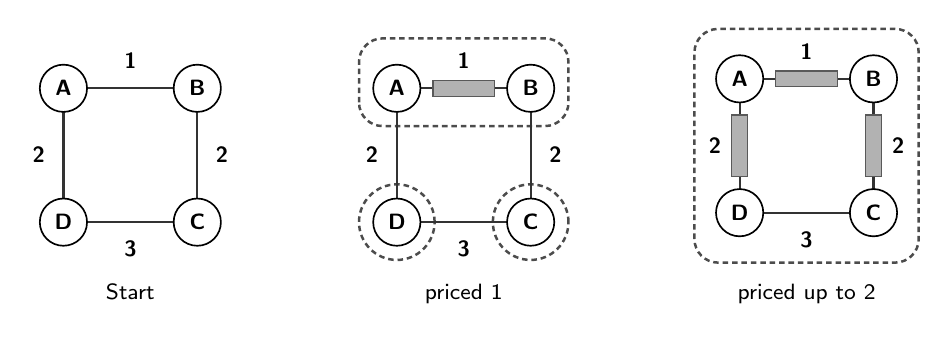
\begin{tikzpicture}[x=1mm,y=1mm]
\draw[line width=0.8pt, black!80] (4.54,27.14) -- (21.54,27.14);
\draw[line width=0.8pt, black!80] (21.54,27.14) -- (21.54,10.14);
\draw[line width=0.8pt, black!80] (21.54,10.14) -- (4.54,10.14);
\draw[line width=0.8pt, black!80] (4.54,10.14) -- (4.54,27.14);
\node[fill=white, inner sep=0, minimum width=2.80mm, minimum height=3.40mm, font=\footnotesize\bfseries] at (13.04,30.58) {1};
\node[fill=white, inner sep=0, minimum width=2.80mm, minimum height=3.40mm, font=\footnotesize\bfseries] at (24.68,18.64) {2};
\node[fill=white, inner sep=0, minimum width=2.80mm, minimum height=3.40mm, font=\footnotesize\bfseries] at (13.04,6.70) {3};
\node[fill=white, inner sep=0, minimum width=2.80mm, minimum height=3.40mm, font=\footnotesize\bfseries] at (1.40,18.64) {2};
\node[circle, draw, line width=0.6pt, fill=white, minimum size=6.00mm, inner sep=0, font=\footnotesize\bfseries] at (4.54,27.14) {A};
\node[circle, draw, line width=0.6pt, fill=white, minimum size=6.00mm, inner sep=0, font=\footnotesize\bfseries] at (21.54,27.14) {B};
\node[circle, draw, line width=0.6pt, fill=white, minimum size=6.00mm, inner sep=0, font=\footnotesize\bfseries] at (21.54,10.14) {C};
\node[circle, draw, line width=0.6pt, fill=white, minimum size=6.00mm, inner sep=0, font=\footnotesize\bfseries] at (4.54,10.14) {D};
\node[font=\footnotesize, anchor=north, align=center] at (13.04,3.50) {Start};
\draw[black!70, line width=0.9pt, dash pattern=on 2pt off 1.4pt, rounded corners=3mm] (42.08,22.34) rectangle (68.68,33.48);
\draw[black!70, line width=0.9pt, dash pattern=on 2pt off 1.4pt] (63.88,10.14) circle (4.80mm);
\draw[black!70, line width=0.9pt, dash pattern=on 2pt off 1.4pt] (46.88,10.14) circle (4.80mm);
\draw[line width=0.8pt, black!80] (46.88,27.14) -- (63.88,27.14);
\draw[line width=0.8pt, black!80] (63.88,27.14) -- (63.88,10.14);
\draw[line width=0.8pt, black!80] (63.88,10.14) -- (46.88,10.14);
\draw[line width=0.8pt, black!80] (46.88,10.14) -- (46.88,27.14);
\filldraw[fill=black!30, draw=black!65, line width=0.4pt] (51.47,28.14) -- (59.29,28.14) -- (59.29,26.14) -- (51.47,26.14) -- cycle;
\node[fill=white, inner sep=0, minimum width=2.80mm, minimum height=3.40mm, font=\footnotesize\bfseries] at (55.38,30.58) {1};
\node[fill=white, inner sep=0, minimum width=2.80mm, minimum height=3.40mm, font=\footnotesize\bfseries] at (67.02,18.64) {2};
\node[fill=white, inner sep=0, minimum width=2.80mm, minimum height=3.40mm, font=\footnotesize\bfseries] at (55.38,6.70) {3};
\node[fill=white, inner sep=0, minimum width=2.80mm, minimum height=3.40mm, font=\footnotesize\bfseries] at (43.74,18.64) {2};
\node[circle, draw, line width=0.6pt, fill=white, minimum size=6.00mm, inner sep=0, font=\footnotesize\bfseries] at (46.88,27.14) {A};
\node[circle, draw, line width=0.6pt, fill=white, minimum size=6.00mm, inner sep=0, font=\footnotesize\bfseries] at (63.88,27.14) {B};
\node[circle, draw, line width=0.6pt, fill=white, minimum size=6.00mm, inner sep=0, font=\footnotesize\bfseries] at (63.88,10.14) {C};
\node[circle, draw, line width=0.6pt, fill=white, minimum size=6.00mm, inner sep=0, font=\footnotesize\bfseries] at (46.88,10.14) {D};
\node[font=\footnotesize, anchor=north, align=center] at (55.38,3.50) {priced 1};
\draw[black!70, line width=0.9pt, dash pattern=on 2pt off 1.4pt, rounded corners=3mm] (84.68,5.00) rectangle (113.16,34.68);
\draw[line width=0.8pt, black!80] (90.42,28.34) -- (107.42,28.34);
\draw[line width=0.8pt, black!80] (107.42,28.34) -- (107.42,11.34);
\draw[line width=0.8pt, black!80] (107.42,11.34) -- (90.42,11.34);
\draw[line width=0.8pt, black!80] (90.42,11.34) -- (90.42,28.34);
\filldraw[fill=black!30, draw=black!65, line width=0.4pt] (95.01,29.34) -- (102.83,29.34) -- (102.83,27.34) -- (95.01,27.34) -- cycle;
\filldraw[fill=black!30, draw=black!65, line width=0.4pt] (108.42,23.75) -- (108.42,15.93) -- (106.42,15.93) -- (106.42,23.75) -- cycle;
\filldraw[fill=black!30, draw=black!65, line width=0.4pt] (89.42,15.93) -- (89.42,23.75) -- (91.42,23.75) -- (91.42,15.93) -- cycle;
\node[fill=white, inner sep=0, minimum width=2.80mm, minimum height=3.40mm, font=\footnotesize\bfseries] at (98.92,31.78) {1};
\node[fill=white, inner sep=0, minimum width=2.80mm, minimum height=3.40mm, font=\footnotesize\bfseries] at (110.56,19.84) {2};
\node[fill=white, inner sep=0, minimum width=2.80mm, minimum height=3.40mm, font=\footnotesize\bfseries] at (98.92,7.90) {3};
\node[fill=white, inner sep=0, minimum width=2.80mm, minimum height=3.40mm, font=\footnotesize\bfseries] at (87.28,19.84) {2};
\node[circle, draw, line width=0.6pt, fill=white, minimum size=6.00mm, inner sep=0, font=\footnotesize\bfseries] at (90.42,28.34) {A};
\node[circle, draw, line width=0.6pt, fill=white, minimum size=6.00mm, inner sep=0, font=\footnotesize\bfseries] at (107.42,28.34) {B};
\node[circle, draw, line width=0.6pt, fill=white, minimum size=6.00mm, inner sep=0, font=\footnotesize\bfseries] at (107.42,11.34) {C};
\node[circle, draw, line width=0.6pt, fill=white, minimum size=6.00mm, inner sep=0, font=\footnotesize\bfseries] at (90.42,11.34) {D};
\node[font=\footnotesize, anchor=north, align=center] at (98.92,3.50) {priced up to 2};
\end{tikzpicture}
\end{center}\par

\par\begin{center}
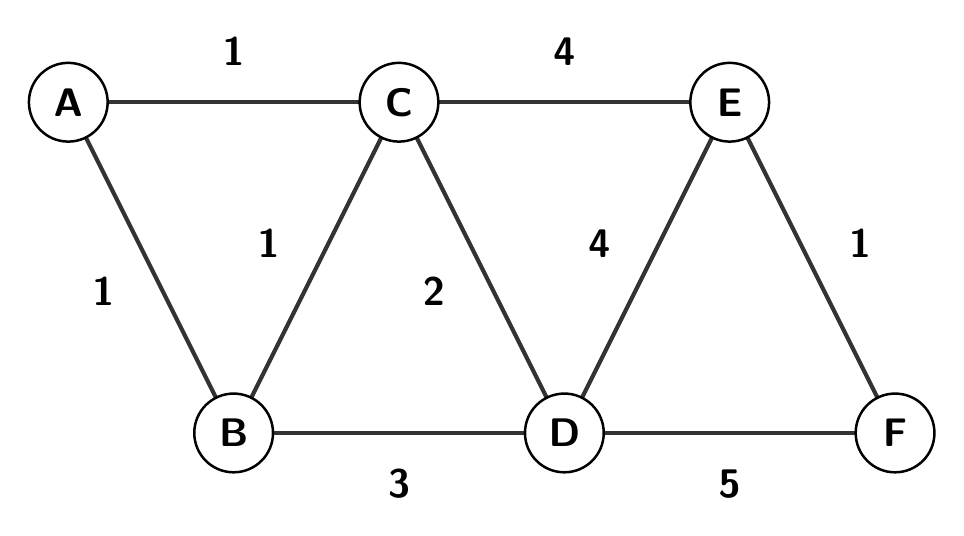
\begin{tikzpicture}[x=1mm,y=1mm]
\draw[line width=1.5pt, black!80] (5.00,51.46) -- (26.00,9.46);
\draw[line width=1.5pt, black!80] (5.00,51.46) -- (47.00,51.46);
\draw[line width=1.5pt, black!80] (26.00,9.46) -- (47.00,51.46);
\draw[line width=1.5pt, black!80] (47.00,51.46) -- (68.00,9.46);
\draw[line width=1.5pt, black!80] (26.00,9.46) -- (68.00,9.46);
\draw[line width=1.5pt, black!80] (47.00,51.46) -- (89.00,51.46);
\draw[line width=1.5pt, black!80] (68.00,9.46) -- (89.00,51.46);
\draw[line width=1.5pt, black!80] (89.00,51.46) -- (110.00,9.46);
\draw[line width=1.5pt, black!80] (68.00,9.46) -- (110.00,9.46);
\node[fill=white, inner sep=0, minimum width=4.40mm, minimum height=6.00mm, font=\Large\bfseries] at (9.44,27.44) {1};
\node[fill=white, inner sep=0, minimum width=4.40mm, minimum height=6.00mm, font=\Large\bfseries] at (26.00,57.93) {1};
\node[fill=white, inner sep=0, minimum width=4.40mm, minimum height=6.00mm, font=\Large\bfseries] at (30.44,33.49) {1};
\node[fill=white, inner sep=0, minimum width=4.40mm, minimum height=6.00mm, font=\Large\bfseries] at (51.44,27.44) {2};
\node[fill=white, inner sep=0, minimum width=4.40mm, minimum height=6.00mm, font=\Large\bfseries] at (47.00,3.00) {3};
\node[fill=white, inner sep=0, minimum width=4.40mm, minimum height=6.00mm, font=\Large\bfseries] at (68.00,57.93) {4};
\node[fill=white, inner sep=0, minimum width=4.40mm, minimum height=6.00mm, font=\Large\bfseries] at (72.44,33.49) {4};
\node[fill=white, inner sep=0, minimum width=4.40mm, minimum height=6.00mm, font=\Large\bfseries] at (105.56,33.49) {1};
\node[fill=white, inner sep=0, minimum width=4.40mm, minimum height=6.00mm, font=\Large\bfseries] at (89.00,3.00) {5};
\node[circle, draw, line width=0.9pt, fill=white, minimum size=10.00mm, inner sep=0, font=\Large\bfseries] at (5.00,51.46) {A};
\node[circle, draw, line width=0.9pt, fill=white, minimum size=10.00mm, inner sep=0, font=\Large\bfseries] at (47.00,51.46) {C};
\node[circle, draw, line width=0.9pt, fill=white, minimum size=10.00mm, inner sep=0, font=\Large\bfseries] at (89.00,51.46) {E};
\node[circle, draw, line width=0.9pt, fill=white, minimum size=10.00mm, inner sep=0, font=\Large\bfseries] at (26.00,9.46) {B};
\node[circle, draw, line width=0.9pt, fill=white, minimum size=10.00mm, inner sep=0, font=\Large\bfseries] at (68.00,9.46) {D};
\node[circle, draw, line width=0.9pt, fill=white, minimum size=10.00mm, inner sep=0, font=\Large\bfseries] at (110.00,9.46) {F};
\end{tikzpicture}
\end{center}\par

\par\begin{center}
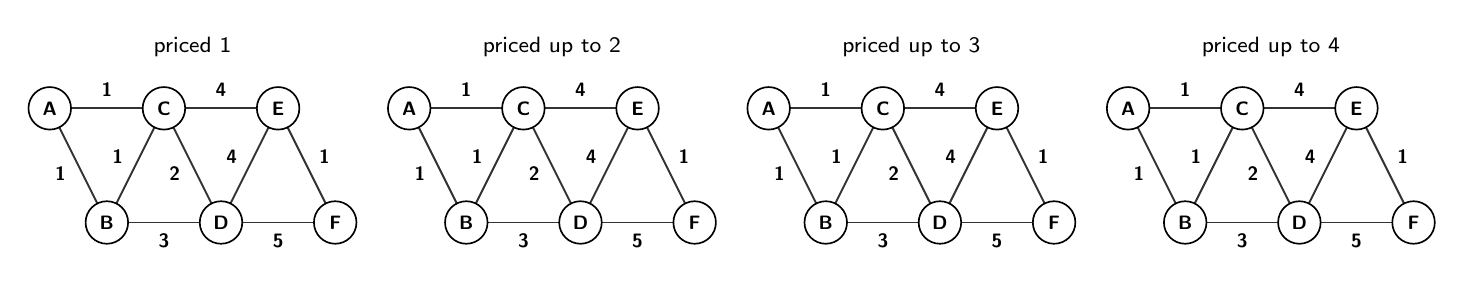
\begin{tikzpicture}[x=1mm,y=1mm]
\draw[line width=0.7pt, black!80] (2.70,18.32) -- (9.95,3.82);
\draw[line width=0.7pt, black!80] (2.70,18.32) -- (17.20,18.32);
\draw[line width=0.7pt, black!80] (9.95,3.82) -- (17.20,18.32);
\draw[line width=0.7pt, black!80] (17.20,18.32) -- (24.45,3.82);
\draw[line width=0.7pt, black!80] (9.95,3.82) -- (24.45,3.82);
\draw[line width=0.7pt, black!80] (17.20,18.32) -- (31.70,18.32);
\draw[line width=0.7pt, black!80] (24.45,3.82) -- (31.70,18.32);
\draw[line width=0.7pt, black!80] (31.70,18.32) -- (38.95,3.82);
\draw[line width=0.7pt, black!80] (24.45,3.82) -- (38.95,3.82);
\node[fill=white, inner sep=0, minimum width=2.30mm, minimum height=3.00mm, font=\scriptsize\bfseries] at (4.07,9.95) {1};
\node[fill=white, inner sep=0, minimum width=2.30mm, minimum height=3.00mm, font=\scriptsize\bfseries] at (9.95,20.65) {1};
\node[fill=white, inner sep=0, minimum width=2.30mm, minimum height=3.00mm, font=\scriptsize\bfseries] at (11.32,12.20) {1};
\node[fill=white, inner sep=0, minimum width=2.30mm, minimum height=3.00mm, font=\scriptsize\bfseries] at (18.57,9.95) {2};
\node[fill=white, inner sep=0, minimum width=2.30mm, minimum height=3.00mm, font=\scriptsize\bfseries] at (17.20,1.50) {3};
\node[fill=white, inner sep=0, minimum width=2.30mm, minimum height=3.00mm, font=\scriptsize\bfseries] at (24.45,20.65) {4};
\node[fill=white, inner sep=0, minimum width=2.30mm, minimum height=3.00mm, font=\scriptsize\bfseries] at (25.82,12.20) {4};
\node[fill=white, inner sep=0, minimum width=2.30mm, minimum height=3.00mm, font=\scriptsize\bfseries] at (37.58,12.20) {1};
\node[fill=white, inner sep=0, minimum width=2.30mm, minimum height=3.00mm, font=\scriptsize\bfseries] at (31.70,1.50) {5};
\node[circle, draw, line width=0.6pt, fill=white, minimum size=5.40mm, inner sep=0, font=\scriptsize\bfseries] at (2.70,18.32) {A};
\node[circle, draw, line width=0.6pt, fill=white, minimum size=5.40mm, inner sep=0, font=\scriptsize\bfseries] at (17.20,18.32) {C};
\node[circle, draw, line width=0.6pt, fill=white, minimum size=5.40mm, inner sep=0, font=\scriptsize\bfseries] at (31.70,18.32) {E};
\node[circle, draw, line width=0.6pt, fill=white, minimum size=5.40mm, inner sep=0, font=\scriptsize\bfseries] at (9.95,3.82) {B};
\node[circle, draw, line width=0.6pt, fill=white, minimum size=5.40mm, inner sep=0, font=\scriptsize\bfseries] at (24.45,3.82) {D};
\node[circle, draw, line width=0.6pt, fill=white, minimum size=5.40mm, inner sep=0, font=\scriptsize\bfseries] at (38.95,3.82) {F};
\node[font=\footnotesize, anchor=south, align=center] at (20.83,23.65) {priced 1};
\draw[line width=0.7pt, black!80] (48.35,18.32) -- (55.60,3.82);
\draw[line width=0.7pt, black!80] (48.35,18.32) -- (62.85,18.32);
\draw[line width=0.7pt, black!80] (55.60,3.82) -- (62.85,18.32);
\draw[line width=0.7pt, black!80] (62.85,18.32) -- (70.10,3.82);
\draw[line width=0.7pt, black!80] (55.60,3.82) -- (70.10,3.82);
\draw[line width=0.7pt, black!80] (62.85,18.32) -- (77.35,18.32);
\draw[line width=0.7pt, black!80] (70.10,3.82) -- (77.35,18.32);
\draw[line width=0.7pt, black!80] (77.35,18.32) -- (84.60,3.82);
\draw[line width=0.7pt, black!80] (70.10,3.82) -- (84.60,3.82);
\node[fill=white, inner sep=0, minimum width=2.30mm, minimum height=3.00mm, font=\scriptsize\bfseries] at (49.72,9.95) {1};
\node[fill=white, inner sep=0, minimum width=2.30mm, minimum height=3.00mm, font=\scriptsize\bfseries] at (55.60,20.65) {1};
\node[fill=white, inner sep=0, minimum width=2.30mm, minimum height=3.00mm, font=\scriptsize\bfseries] at (56.97,12.20) {1};
\node[fill=white, inner sep=0, minimum width=2.30mm, minimum height=3.00mm, font=\scriptsize\bfseries] at (64.22,9.95) {2};
\node[fill=white, inner sep=0, minimum width=2.30mm, minimum height=3.00mm, font=\scriptsize\bfseries] at (62.85,1.50) {3};
\node[fill=white, inner sep=0, minimum width=2.30mm, minimum height=3.00mm, font=\scriptsize\bfseries] at (70.10,20.65) {4};
\node[fill=white, inner sep=0, minimum width=2.30mm, minimum height=3.00mm, font=\scriptsize\bfseries] at (71.47,12.20) {4};
\node[fill=white, inner sep=0, minimum width=2.30mm, minimum height=3.00mm, font=\scriptsize\bfseries] at (83.23,12.20) {1};
\node[fill=white, inner sep=0, minimum width=2.30mm, minimum height=3.00mm, font=\scriptsize\bfseries] at (77.35,1.50) {5};
\node[circle, draw, line width=0.6pt, fill=white, minimum size=5.40mm, inner sep=0, font=\scriptsize\bfseries] at (48.35,18.32) {A};
\node[circle, draw, line width=0.6pt, fill=white, minimum size=5.40mm, inner sep=0, font=\scriptsize\bfseries] at (62.85,18.32) {C};
\node[circle, draw, line width=0.6pt, fill=white, minimum size=5.40mm, inner sep=0, font=\scriptsize\bfseries] at (77.35,18.32) {E};
\node[circle, draw, line width=0.6pt, fill=white, minimum size=5.40mm, inner sep=0, font=\scriptsize\bfseries] at (55.60,3.82) {B};
\node[circle, draw, line width=0.6pt, fill=white, minimum size=5.40mm, inner sep=0, font=\scriptsize\bfseries] at (70.10,3.82) {D};
\node[circle, draw, line width=0.6pt, fill=white, minimum size=5.40mm, inner sep=0, font=\scriptsize\bfseries] at (84.60,3.82) {F};
\node[font=\footnotesize, anchor=south, align=center] at (66.48,23.65) {priced up to 2};
\draw[line width=0.7pt, black!80] (94.00,18.32) -- (101.25,3.82);
\draw[line width=0.7pt, black!80] (94.00,18.32) -- (108.50,18.32);
\draw[line width=0.7pt, black!80] (101.25,3.82) -- (108.50,18.32);
\draw[line width=0.7pt, black!80] (108.50,18.32) -- (115.75,3.82);
\draw[line width=0.7pt, black!80] (101.25,3.82) -- (115.75,3.82);
\draw[line width=0.7pt, black!80] (108.50,18.32) -- (123.00,18.32);
\draw[line width=0.7pt, black!80] (115.75,3.82) -- (123.00,18.32);
\draw[line width=0.7pt, black!80] (123.00,18.32) -- (130.25,3.82);
\draw[line width=0.7pt, black!80] (115.75,3.82) -- (130.25,3.82);
\node[fill=white, inner sep=0, minimum width=2.30mm, minimum height=3.00mm, font=\scriptsize\bfseries] at (95.37,9.95) {1};
\node[fill=white, inner sep=0, minimum width=2.30mm, minimum height=3.00mm, font=\scriptsize\bfseries] at (101.25,20.65) {1};
\node[fill=white, inner sep=0, minimum width=2.30mm, minimum height=3.00mm, font=\scriptsize\bfseries] at (102.62,12.20) {1};
\node[fill=white, inner sep=0, minimum width=2.30mm, minimum height=3.00mm, font=\scriptsize\bfseries] at (109.87,9.95) {2};
\node[fill=white, inner sep=0, minimum width=2.30mm, minimum height=3.00mm, font=\scriptsize\bfseries] at (108.50,1.50) {3};
\node[fill=white, inner sep=0, minimum width=2.30mm, minimum height=3.00mm, font=\scriptsize\bfseries] at (115.75,20.65) {4};
\node[fill=white, inner sep=0, minimum width=2.30mm, minimum height=3.00mm, font=\scriptsize\bfseries] at (117.12,12.20) {4};
\node[fill=white, inner sep=0, minimum width=2.30mm, minimum height=3.00mm, font=\scriptsize\bfseries] at (128.88,12.20) {1};
\node[fill=white, inner sep=0, minimum width=2.30mm, minimum height=3.00mm, font=\scriptsize\bfseries] at (123.00,1.50) {5};
\node[circle, draw, line width=0.6pt, fill=white, minimum size=5.40mm, inner sep=0, font=\scriptsize\bfseries] at (94.00,18.32) {A};
\node[circle, draw, line width=0.6pt, fill=white, minimum size=5.40mm, inner sep=0, font=\scriptsize\bfseries] at (108.50,18.32) {C};
\node[circle, draw, line width=0.6pt, fill=white, minimum size=5.40mm, inner sep=0, font=\scriptsize\bfseries] at (123.00,18.32) {E};
\node[circle, draw, line width=0.6pt, fill=white, minimum size=5.40mm, inner sep=0, font=\scriptsize\bfseries] at (101.25,3.82) {B};
\node[circle, draw, line width=0.6pt, fill=white, minimum size=5.40mm, inner sep=0, font=\scriptsize\bfseries] at (115.75,3.82) {D};
\node[circle, draw, line width=0.6pt, fill=white, minimum size=5.40mm, inner sep=0, font=\scriptsize\bfseries] at (130.25,3.82) {F};
\node[font=\footnotesize, anchor=south, align=center] at (112.13,23.65) {priced up to 3};
\draw[line width=0.7pt, black!80] (139.65,18.32) -- (146.90,3.82);
\draw[line width=0.7pt, black!80] (139.65,18.32) -- (154.15,18.32);
\draw[line width=0.7pt, black!80] (146.90,3.82) -- (154.15,18.32);
\draw[line width=0.7pt, black!80] (154.15,18.32) -- (161.40,3.82);
\draw[line width=0.7pt, black!80] (146.90,3.82) -- (161.40,3.82);
\draw[line width=0.7pt, black!80] (154.15,18.32) -- (168.65,18.32);
\draw[line width=0.7pt, black!80] (161.40,3.82) -- (168.65,18.32);
\draw[line width=0.7pt, black!80] (168.65,18.32) -- (175.90,3.82);
\draw[line width=0.7pt, black!80] (161.40,3.82) -- (175.90,3.82);
\node[fill=white, inner sep=0, minimum width=2.30mm, minimum height=3.00mm, font=\scriptsize\bfseries] at (141.02,9.95) {1};
\node[fill=white, inner sep=0, minimum width=2.30mm, minimum height=3.00mm, font=\scriptsize\bfseries] at (146.90,20.65) {1};
\node[fill=white, inner sep=0, minimum width=2.30mm, minimum height=3.00mm, font=\scriptsize\bfseries] at (148.27,12.20) {1};
\node[fill=white, inner sep=0, minimum width=2.30mm, minimum height=3.00mm, font=\scriptsize\bfseries] at (155.52,9.95) {2};
\node[fill=white, inner sep=0, minimum width=2.30mm, minimum height=3.00mm, font=\scriptsize\bfseries] at (154.15,1.50) {3};
\node[fill=white, inner sep=0, minimum width=2.30mm, minimum height=3.00mm, font=\scriptsize\bfseries] at (161.40,20.65) {4};
\node[fill=white, inner sep=0, minimum width=2.30mm, minimum height=3.00mm, font=\scriptsize\bfseries] at (162.77,12.20) {4};
\node[fill=white, inner sep=0, minimum width=2.30mm, minimum height=3.00mm, font=\scriptsize\bfseries] at (174.53,12.20) {1};
\node[fill=white, inner sep=0, minimum width=2.30mm, minimum height=3.00mm, font=\scriptsize\bfseries] at (168.65,1.50) {5};
\node[circle, draw, line width=0.6pt, fill=white, minimum size=5.40mm, inner sep=0, font=\scriptsize\bfseries] at (139.65,18.32) {A};
\node[circle, draw, line width=0.6pt, fill=white, minimum size=5.40mm, inner sep=0, font=\scriptsize\bfseries] at (154.15,18.32) {C};
\node[circle, draw, line width=0.6pt, fill=white, minimum size=5.40mm, inner sep=0, font=\scriptsize\bfseries] at (168.65,18.32) {E};
\node[circle, draw, line width=0.6pt, fill=white, minimum size=5.40mm, inner sep=0, font=\scriptsize\bfseries] at (146.90,3.82) {B};
\node[circle, draw, line width=0.6pt, fill=white, minimum size=5.40mm, inner sep=0, font=\scriptsize\bfseries] at (161.40,3.82) {D};
\node[circle, draw, line width=0.6pt, fill=white, minimum size=5.40mm, inner sep=0, font=\scriptsize\bfseries] at (175.90,3.82) {F};
\node[font=\footnotesize, anchor=south, align=center] at (157.78,23.65) {priced up to 4};
\end{tikzpicture}
\end{center}\par

\vspace{4mm}
\begin{center}
A and D: \ans{14mm}\hspace{9mm} B and D: \ans{14mm}\hspace{9mm} D and F: \ans{14mm}\hspace{9mm} A and F: \ans{14mm}
\end{center}
\newpage

\prob{4} On a trip, the pawn walks from one place to another along any links, and you pay each link's price every time the pawn walks along it. Write the trip by its letters, and pay when the trip is over.

\par\begin{center}
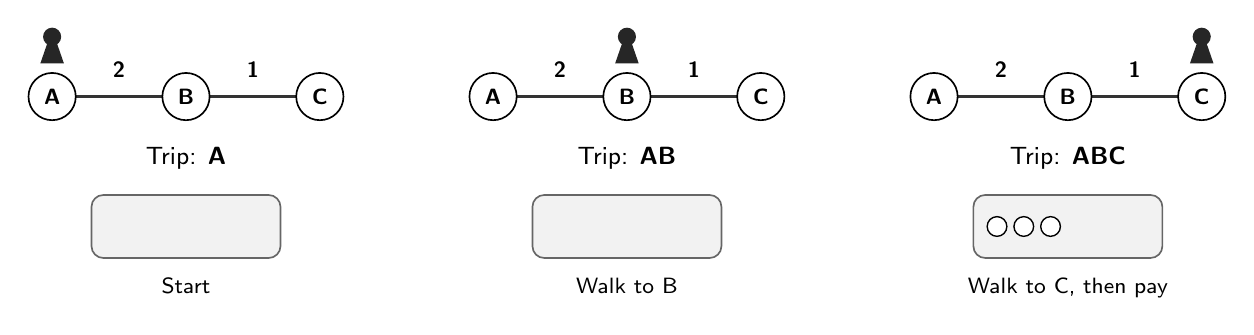
\begin{tikzpicture}[x=1mm,y=1mm]
\draw[line width=0.8pt, black!80] (3.00,25.00) -- (20.00,25.00);
\draw[line width=0.8pt, black!80] (20.00,25.00) -- (37.00,25.00);
\node[fill=white, inner sep=0, minimum width=2.80mm, minimum height=3.40mm, font=\footnotesize\bfseries] at (11.50,28.44) {2};
\node[fill=white, inner sep=0, minimum width=2.80mm, minimum height=3.40mm, font=\footnotesize\bfseries] at (28.50,28.44) {1};
\node[circle, draw, line width=0.6pt, fill=white, minimum size=6.00mm, inner sep=0, font=\footnotesize\bfseries] at (3.00,25.00) {A};
\node[circle, draw, line width=0.6pt, fill=white, minimum size=6.00mm, inner sep=0, font=\footnotesize\bfseries] at (20.00,25.00) {B};
\node[circle, draw, line width=0.6pt, fill=white, minimum size=6.00mm, inner sep=0, font=\footnotesize\bfseries] at (37.00,25.00) {C};
\fill[black!85] (1.50,29.20) -- (4.50,29.20) -- (3.60,31.80) -- (2.40,31.80) -- cycle;\fill[black!85] (3.00,32.60) circle (1.15mm);
\node[font=\small, anchor=south] at (20.00,14.5) {Trip: \textbf{A}};
\draw[black!60, line width=0.6pt, fill=black!5, rounded corners=1.5mm] (8.00,4.50) rectangle (32.00,12.50);
\node[font=\footnotesize, anchor=north, align=center] at (20.00,3.20) {Start};
\draw[line width=0.8pt, black!80] (59.00,25.00) -- (76.00,25.00);
\draw[line width=0.8pt, black!80] (76.00,25.00) -- (93.00,25.00);
\node[fill=white, inner sep=0, minimum width=2.80mm, minimum height=3.40mm, font=\footnotesize\bfseries] at (67.50,28.44) {2};
\node[fill=white, inner sep=0, minimum width=2.80mm, minimum height=3.40mm, font=\footnotesize\bfseries] at (84.50,28.44) {1};
\node[circle, draw, line width=0.6pt, fill=white, minimum size=6.00mm, inner sep=0, font=\footnotesize\bfseries] at (59.00,25.00) {A};
\node[circle, draw, line width=0.6pt, fill=white, minimum size=6.00mm, inner sep=0, font=\footnotesize\bfseries] at (76.00,25.00) {B};
\node[circle, draw, line width=0.6pt, fill=white, minimum size=6.00mm, inner sep=0, font=\footnotesize\bfseries] at (93.00,25.00) {C};
\fill[black!85] (74.50,29.20) -- (77.50,29.20) -- (76.60,31.80) -- (75.40,31.80) -- cycle;\fill[black!85] (76.00,32.60) circle (1.15mm);
\node[font=\small, anchor=south] at (76.00,14.5) {Trip: \textbf{AB}};
\draw[black!60, line width=0.6pt, fill=black!5, rounded corners=1.5mm] (64.00,4.50) rectangle (88.00,12.50);
\node[font=\footnotesize, anchor=north, align=center] at (76.00,3.20) {Walk to B};
\draw[line width=0.8pt, black!80] (115.00,25.00) -- (132.00,25.00);
\draw[line width=0.8pt, black!80] (132.00,25.00) -- (149.00,25.00);
\node[fill=white, inner sep=0, minimum width=2.80mm, minimum height=3.40mm, font=\footnotesize\bfseries] at (123.50,28.44) {2};
\node[fill=white, inner sep=0, minimum width=2.80mm, minimum height=3.40mm, font=\footnotesize\bfseries] at (140.50,28.44) {1};
\node[circle, draw, line width=0.6pt, fill=white, minimum size=6.00mm, inner sep=0, font=\footnotesize\bfseries] at (115.00,25.00) {A};
\node[circle, draw, line width=0.6pt, fill=white, minimum size=6.00mm, inner sep=0, font=\footnotesize\bfseries] at (132.00,25.00) {B};
\node[circle, draw, line width=0.6pt, fill=white, minimum size=6.00mm, inner sep=0, font=\footnotesize\bfseries] at (149.00,25.00) {C};
\fill[black!85] (147.50,29.20) -- (150.50,29.20) -- (149.60,31.80) -- (148.40,31.80) -- cycle;\fill[black!85] (149.00,32.60) circle (1.15mm);
\node[font=\small, anchor=south] at (132.00,14.5) {Trip: \textbf{ABC}};
\draw[black!60, line width=0.6pt, fill=black!5, rounded corners=1.5mm] (120.00,4.50) rectangle (144.00,12.50);
\draw[line width=0.5pt, fill=white] (123.00,8.50) circle (1.25mm);
\draw[line width=0.5pt, fill=white] (126.40,8.50) circle (1.25mm);
\draw[line width=0.5pt, fill=white] (129.80,8.50) circle (1.25mm);
\node[font=\footnotesize, anchor=north, align=center] at (132.00,3.20) {Walk to C, then pay};
\end{tikzpicture}
\end{center}\par

On each map, find the cheapest network and the cheapest trip from A to D.

\vspace{4mm}

\par\begin{center}
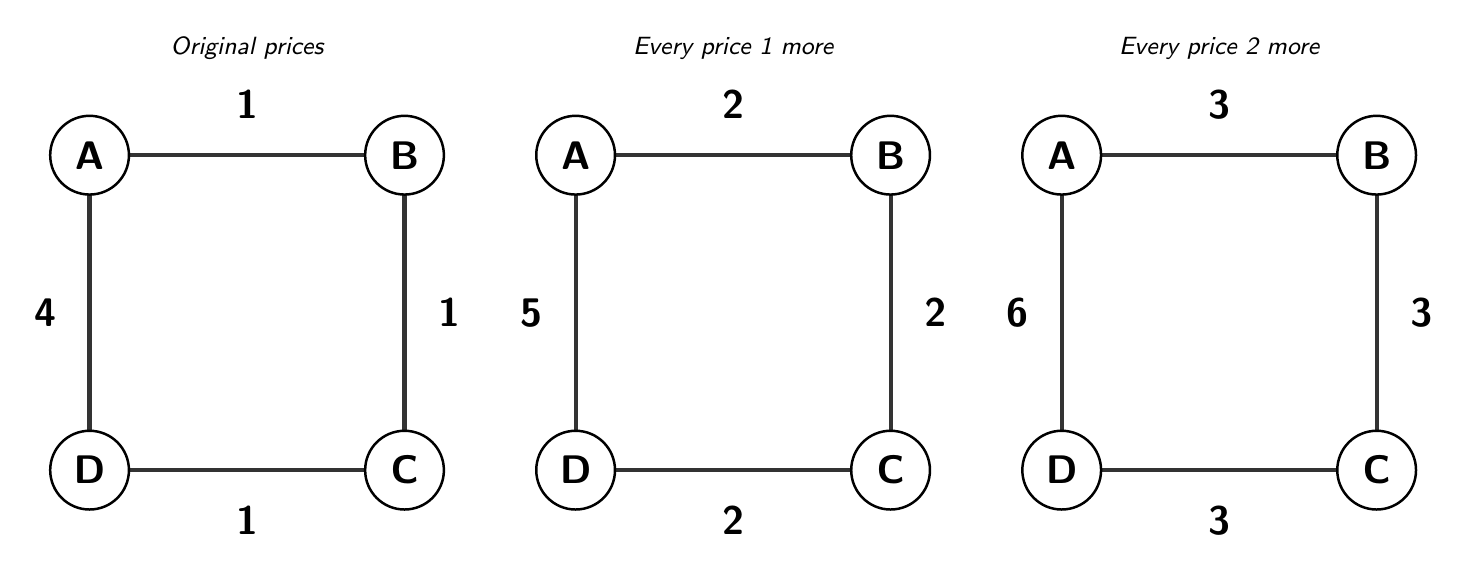
\begin{tikzpicture}[x=1mm,y=1mm]
\draw[line width=1.5pt, black!80] (7.86,49.46) -- (47.86,49.46);
\draw[line width=1.5pt, black!80] (47.86,49.46) -- (47.86,9.46);
\draw[line width=1.5pt, black!80] (47.86,9.46) -- (7.86,9.46);
\draw[line width=1.5pt, black!80] (7.86,9.46) -- (7.86,49.46);
\node[fill=white, inner sep=0, minimum width=4.40mm, minimum height=6.00mm, font=\Large\bfseries] at (27.86,55.93) {1};
\node[fill=white, inner sep=0, minimum width=4.40mm, minimum height=6.00mm, font=\Large\bfseries] at (53.53,29.46) {1};
\node[fill=white, inner sep=0, minimum width=4.40mm, minimum height=6.00mm, font=\Large\bfseries] at (27.86,3.00) {1};
\node[fill=white, inner sep=0, minimum width=4.40mm, minimum height=6.00mm, font=\Large\bfseries] at (2.20,29.46) {4};
\node[circle, draw, line width=0.9pt, fill=white, minimum size=10.00mm, inner sep=0, font=\Large\bfseries] at (7.86,49.46) {A};
\node[circle, draw, line width=0.9pt, fill=white, minimum size=10.00mm, inner sep=0, font=\Large\bfseries] at (47.86,49.46) {B};
\node[circle, draw, line width=0.9pt, fill=white, minimum size=10.00mm, inner sep=0, font=\Large\bfseries] at (47.86,9.46) {C};
\node[circle, draw, line width=0.9pt, fill=white, minimum size=10.00mm, inner sep=0, font=\Large\bfseries] at (7.86,9.46) {D};
\node[font=\small, anchor=south, align=center] at (27.86,60.43) {\itshape Original prices};
\draw[line width=1.5pt, black!80] (69.59,49.46) -- (109.59,49.46);
\draw[line width=1.5pt, black!80] (109.59,49.46) -- (109.59,9.46);
\draw[line width=1.5pt, black!80] (109.59,9.46) -- (69.59,9.46);
\draw[line width=1.5pt, black!80] (69.59,9.46) -- (69.59,49.46);
\node[fill=white, inner sep=0, minimum width=4.40mm, minimum height=6.00mm, font=\Large\bfseries] at (89.59,55.93) {2};
\node[fill=white, inner sep=0, minimum width=4.40mm, minimum height=6.00mm, font=\Large\bfseries] at (115.26,29.46) {2};
\node[fill=white, inner sep=0, minimum width=4.40mm, minimum height=6.00mm, font=\Large\bfseries] at (89.59,3.00) {2};
\node[fill=white, inner sep=0, minimum width=4.40mm, minimum height=6.00mm, font=\Large\bfseries] at (63.93,29.46) {5};
\node[circle, draw, line width=0.9pt, fill=white, minimum size=10.00mm, inner sep=0, font=\Large\bfseries] at (69.59,49.46) {A};
\node[circle, draw, line width=0.9pt, fill=white, minimum size=10.00mm, inner sep=0, font=\Large\bfseries] at (109.59,49.46) {B};
\node[circle, draw, line width=0.9pt, fill=white, minimum size=10.00mm, inner sep=0, font=\Large\bfseries] at (109.59,9.46) {C};
\node[circle, draw, line width=0.9pt, fill=white, minimum size=10.00mm, inner sep=0, font=\Large\bfseries] at (69.59,9.46) {D};
\node[font=\small, anchor=south, align=center] at (89.59,60.43) {\itshape Every price 1 more};
\draw[line width=1.5pt, black!80] (131.32,49.46) -- (171.32,49.46);
\draw[line width=1.5pt, black!80] (171.32,49.46) -- (171.32,9.46);
\draw[line width=1.5pt, black!80] (171.32,9.46) -- (131.32,9.46);
\draw[line width=1.5pt, black!80] (131.32,9.46) -- (131.32,49.46);
\node[fill=white, inner sep=0, minimum width=4.40mm, minimum height=6.00mm, font=\Large\bfseries] at (151.32,55.93) {3};
\node[fill=white, inner sep=0, minimum width=4.40mm, minimum height=6.00mm, font=\Large\bfseries] at (176.99,29.46) {3};
\node[fill=white, inner sep=0, minimum width=4.40mm, minimum height=6.00mm, font=\Large\bfseries] at (151.32,3.00) {3};
\node[fill=white, inner sep=0, minimum width=4.40mm, minimum height=6.00mm, font=\Large\bfseries] at (125.66,29.46) {6};
\node[circle, draw, line width=0.9pt, fill=white, minimum size=10.00mm, inner sep=0, font=\Large\bfseries] at (131.32,49.46) {A};
\node[circle, draw, line width=0.9pt, fill=white, minimum size=10.00mm, inner sep=0, font=\Large\bfseries] at (171.32,49.46) {B};
\node[circle, draw, line width=0.9pt, fill=white, minimum size=10.00mm, inner sep=0, font=\Large\bfseries] at (171.32,9.46) {C};
\node[circle, draw, line width=0.9pt, fill=white, minimum size=10.00mm, inner sep=0, font=\Large\bfseries] at (131.32,9.46) {D};
\node[font=\small, anchor=south, align=center] at (151.32,60.43) {\itshape Every price 2 more};
\end{tikzpicture}
\end{center}\par

\vspace{3mm}
\begin{center}
\begin{minipage}[t]{58mm}\small
Network \ans{40mm}\\[1.5mm]
costs \ans{12mm}\\[7mm]
Trip \ans{44mm}\\[1.5mm]
costs \ans{12mm}
\end{minipage}\hfill\begin{minipage}[t]{58mm}\small
Network \ans{40mm}\\[1.5mm]
costs \ans{12mm}\\[7mm]
Trip \ans{44mm}\\[1.5mm]
costs \ans{12mm}
\end{minipage}\hfill\begin{minipage}[t]{58mm}\small
Network \ans{40mm}\\[1.5mm]
costs \ans{12mm}\\[7mm]
Trip \ans{44mm}\\[1.5mm]
costs \ans{12mm}
\end{minipage}
\end{center}
\newpage

\prob{5} On each map, find the cheapest network and every cheapest trip from A to F.

\vspace{3mm}

\noindent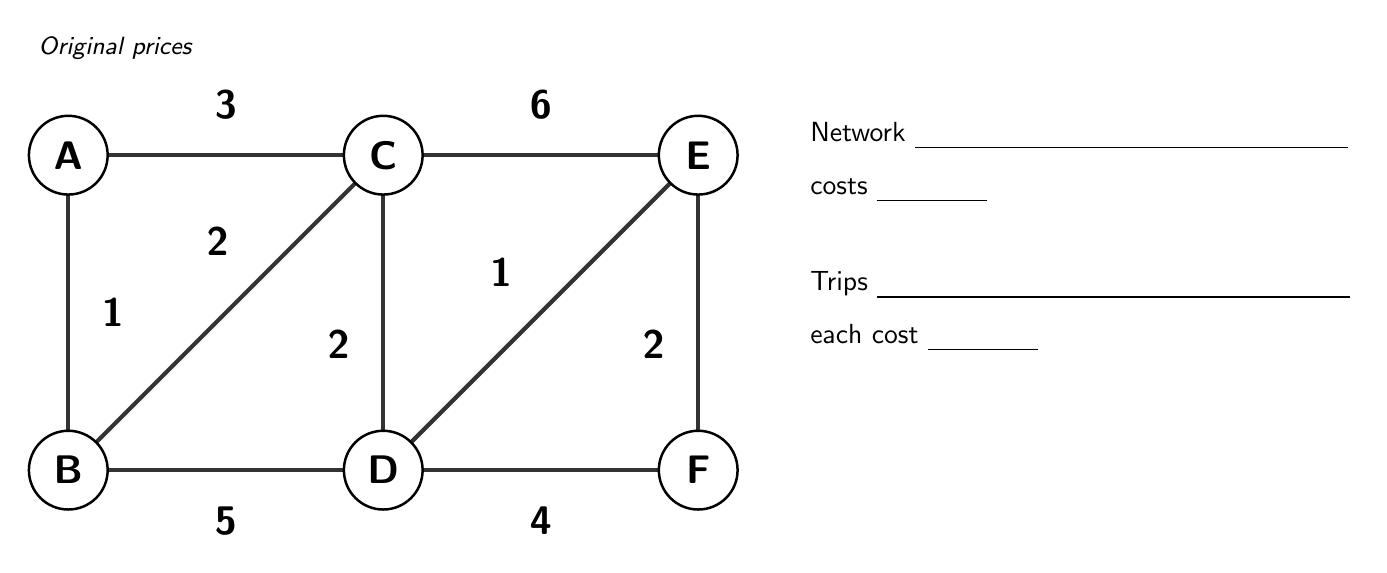
\begin{tikzpicture}[x=1mm,y=1mm]
\draw[line width=1.5pt, black!80] (5.00,49.46) -- (5.00,9.46);
\draw[line width=1.5pt, black!80] (5.00,9.46) -- (45.00,49.46);
\draw[line width=1.5pt, black!80] (5.00,49.46) -- (45.00,49.46);
\draw[line width=1.5pt, black!80] (45.00,49.46) -- (45.00,9.46);
\draw[line width=1.5pt, black!80] (45.00,9.46) -- (85.00,49.46);
\draw[line width=1.5pt, black!80] (85.00,49.46) -- (85.00,9.46);
\draw[line width=1.5pt, black!80] (45.00,9.46) -- (85.00,9.46);
\draw[line width=1.5pt, black!80] (5.00,9.46) -- (45.00,9.46);
\draw[line width=1.5pt, black!80] (45.00,49.46) -- (85.00,49.46);
\node[fill=white, inner sep=0, minimum width=4.40mm, minimum height=6.00mm, font=\Large\bfseries] at (10.66,29.46) {1};
\node[fill=white, inner sep=0, minimum width=4.40mm, minimum height=6.00mm, font=\Large\bfseries] at (23.95,38.51) {2};
\node[fill=white, inner sep=0, minimum width=4.40mm, minimum height=6.00mm, font=\Large\bfseries] at (25.00,55.93) {3};
\node[fill=white, inner sep=0, minimum width=4.40mm, minimum height=6.00mm, font=\Large\bfseries] at (39.34,25.46) {2};
\node[fill=white, inner sep=0, minimum width=4.40mm, minimum height=6.00mm, font=\Large\bfseries] at (59.95,34.51) {1};
\node[fill=white, inner sep=0, minimum width=4.40mm, minimum height=6.00mm, font=\Large\bfseries] at (79.34,25.46) {2};
\node[fill=white, inner sep=0, minimum width=4.40mm, minimum height=6.00mm, font=\Large\bfseries] at (65.00,3.00) {4};
\node[fill=white, inner sep=0, minimum width=4.40mm, minimum height=6.00mm, font=\Large\bfseries] at (25.00,3.00) {5};
\node[fill=white, inner sep=0, minimum width=4.40mm, minimum height=6.00mm, font=\Large\bfseries] at (65.00,55.93) {6};
\node[circle, draw, line width=0.9pt, fill=white, minimum size=10.00mm, inner sep=0, font=\Large\bfseries] at (5.00,49.46) {A};
\node[circle, draw, line width=0.9pt, fill=white, minimum size=10.00mm, inner sep=0, font=\Large\bfseries] at (45.00,49.46) {C};
\node[circle, draw, line width=0.9pt, fill=white, minimum size=10.00mm, inner sep=0, font=\Large\bfseries] at (85.00,49.46) {E};
\node[circle, draw, line width=0.9pt, fill=white, minimum size=10.00mm, inner sep=0, font=\Large\bfseries] at (5.00,9.46) {B};
\node[circle, draw, line width=0.9pt, fill=white, minimum size=10.00mm, inner sep=0, font=\Large\bfseries] at (45.00,9.46) {D};
\node[circle, draw, line width=0.9pt, fill=white, minimum size=10.00mm, inner sep=0, font=\Large\bfseries] at (85.00,9.46) {F};
\node[anchor=north west, font=\normalsize, align=left] at (98.00,54.93) {Network \ans{55mm}\\[2.5mm] costs \ans{14mm}\\[8mm] Trips \ans{60mm}\\[2.5mm] each cost \ans{14mm}};
\node[anchor=south west, font=\small\itshape] at (0,60.43) {Original prices};
\end{tikzpicture}\par\vspace{5mm}

\noindent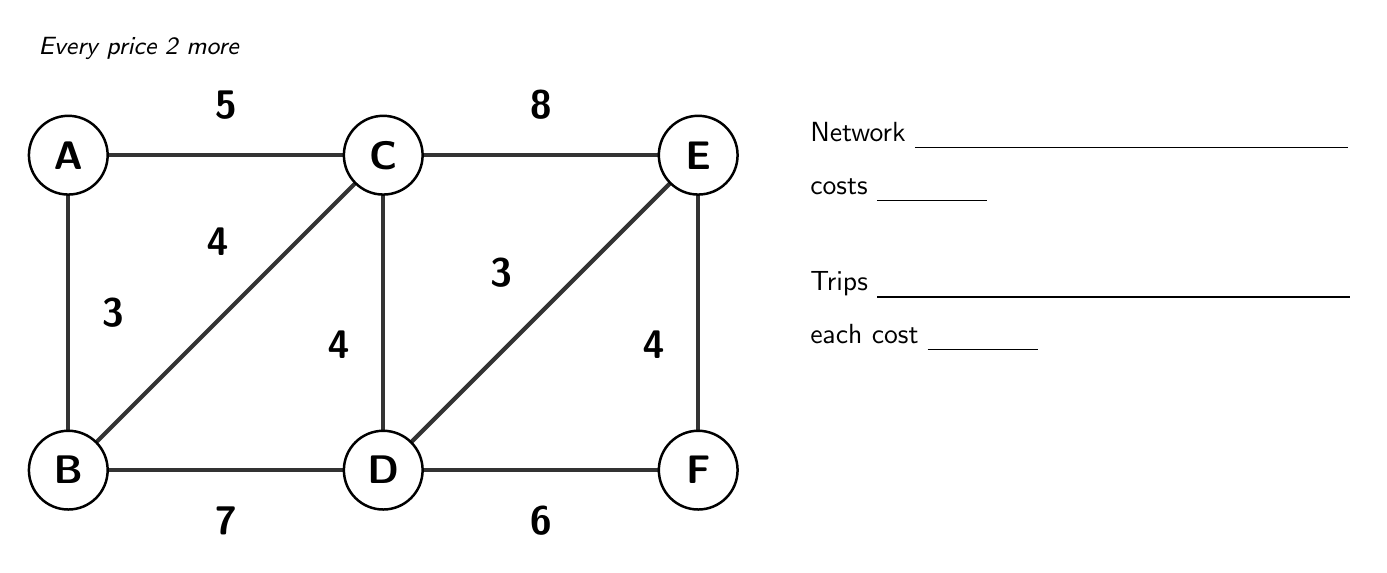
\begin{tikzpicture}[x=1mm,y=1mm]
\draw[line width=1.5pt, black!80] (5.00,49.46) -- (5.00,9.46);
\draw[line width=1.5pt, black!80] (5.00,9.46) -- (45.00,49.46);
\draw[line width=1.5pt, black!80] (5.00,49.46) -- (45.00,49.46);
\draw[line width=1.5pt, black!80] (45.00,49.46) -- (45.00,9.46);
\draw[line width=1.5pt, black!80] (45.00,9.46) -- (85.00,49.46);
\draw[line width=1.5pt, black!80] (85.00,49.46) -- (85.00,9.46);
\draw[line width=1.5pt, black!80] (45.00,9.46) -- (85.00,9.46);
\draw[line width=1.5pt, black!80] (5.00,9.46) -- (45.00,9.46);
\draw[line width=1.5pt, black!80] (45.00,49.46) -- (85.00,49.46);
\node[fill=white, inner sep=0, minimum width=4.40mm, minimum height=6.00mm, font=\Large\bfseries] at (10.66,29.46) {3};
\node[fill=white, inner sep=0, minimum width=4.40mm, minimum height=6.00mm, font=\Large\bfseries] at (23.95,38.51) {4};
\node[fill=white, inner sep=0, minimum width=4.40mm, minimum height=6.00mm, font=\Large\bfseries] at (25.00,55.93) {5};
\node[fill=white, inner sep=0, minimum width=4.40mm, minimum height=6.00mm, font=\Large\bfseries] at (39.34,25.46) {4};
\node[fill=white, inner sep=0, minimum width=4.40mm, minimum height=6.00mm, font=\Large\bfseries] at (59.95,34.51) {3};
\node[fill=white, inner sep=0, minimum width=4.40mm, minimum height=6.00mm, font=\Large\bfseries] at (79.34,25.46) {4};
\node[fill=white, inner sep=0, minimum width=4.40mm, minimum height=6.00mm, font=\Large\bfseries] at (65.00,3.00) {6};
\node[fill=white, inner sep=0, minimum width=4.40mm, minimum height=6.00mm, font=\Large\bfseries] at (25.00,3.00) {7};
\node[fill=white, inner sep=0, minimum width=4.40mm, minimum height=6.00mm, font=\Large\bfseries] at (65.00,55.93) {8};
\node[circle, draw, line width=0.9pt, fill=white, minimum size=10.00mm, inner sep=0, font=\Large\bfseries] at (5.00,49.46) {A};
\node[circle, draw, line width=0.9pt, fill=white, minimum size=10.00mm, inner sep=0, font=\Large\bfseries] at (45.00,49.46) {C};
\node[circle, draw, line width=0.9pt, fill=white, minimum size=10.00mm, inner sep=0, font=\Large\bfseries] at (85.00,49.46) {E};
\node[circle, draw, line width=0.9pt, fill=white, minimum size=10.00mm, inner sep=0, font=\Large\bfseries] at (5.00,9.46) {B};
\node[circle, draw, line width=0.9pt, fill=white, minimum size=10.00mm, inner sep=0, font=\Large\bfseries] at (45.00,9.46) {D};
\node[circle, draw, line width=0.9pt, fill=white, minimum size=10.00mm, inner sep=0, font=\Large\bfseries] at (85.00,9.46) {F};
\node[anchor=north west, font=\normalsize, align=left] at (98.00,54.93) {Network \ans{55mm}\\[2.5mm] costs \ans{14mm}\\[8mm] Trips \ans{60mm}\\[2.5mm] each cost \ans{14mm}};
\node[anchor=south west, font=\small\itshape] at (0,60.43) {Every price 2 more};
\end{tikzpicture}\par\vspace{5mm}

\noindent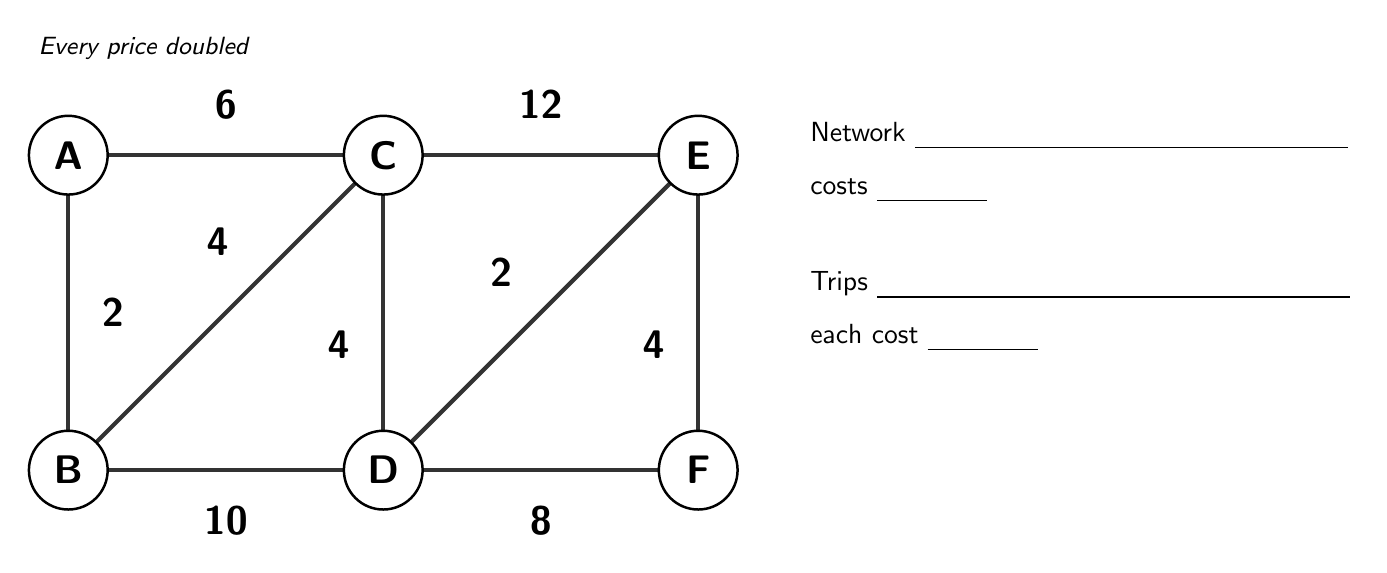
\begin{tikzpicture}[x=1mm,y=1mm]
\draw[line width=1.5pt, black!80] (5.00,49.46) -- (5.00,9.46);
\draw[line width=1.5pt, black!80] (5.00,9.46) -- (45.00,49.46);
\draw[line width=1.5pt, black!80] (5.00,49.46) -- (45.00,49.46);
\draw[line width=1.5pt, black!80] (45.00,49.46) -- (45.00,9.46);
\draw[line width=1.5pt, black!80] (45.00,9.46) -- (85.00,49.46);
\draw[line width=1.5pt, black!80] (85.00,49.46) -- (85.00,9.46);
\draw[line width=1.5pt, black!80] (45.00,9.46) -- (85.00,9.46);
\draw[line width=1.5pt, black!80] (5.00,9.46) -- (45.00,9.46);
\draw[line width=1.5pt, black!80] (45.00,49.46) -- (85.00,49.46);
\node[fill=white, inner sep=0, minimum width=4.40mm, minimum height=6.00mm, font=\Large\bfseries] at (10.66,29.46) {2};
\node[fill=white, inner sep=0, minimum width=4.40mm, minimum height=6.00mm, font=\Large\bfseries] at (23.95,38.51) {4};
\node[fill=white, inner sep=0, minimum width=4.40mm, minimum height=6.00mm, font=\Large\bfseries] at (25.00,55.93) {6};
\node[fill=white, inner sep=0, minimum width=4.40mm, minimum height=6.00mm, font=\Large\bfseries] at (39.34,25.46) {4};
\node[fill=white, inner sep=0, minimum width=4.40mm, minimum height=6.00mm, font=\Large\bfseries] at (59.95,34.51) {2};
\node[fill=white, inner sep=0, minimum width=4.40mm, minimum height=6.00mm, font=\Large\bfseries] at (79.34,25.46) {4};
\node[fill=white, inner sep=0, minimum width=4.40mm, minimum height=6.00mm, font=\Large\bfseries] at (65.00,3.00) {8};
\node[fill=white, inner sep=0, minimum width=7.60mm, minimum height=6.00mm, font=\Large\bfseries] at (25.00,3.00) {10};
\node[fill=white, inner sep=0, minimum width=7.60mm, minimum height=6.00mm, font=\Large\bfseries] at (65.00,55.93) {12};
\node[circle, draw, line width=0.9pt, fill=white, minimum size=10.00mm, inner sep=0, font=\Large\bfseries] at (5.00,49.46) {A};
\node[circle, draw, line width=0.9pt, fill=white, minimum size=10.00mm, inner sep=0, font=\Large\bfseries] at (45.00,49.46) {C};
\node[circle, draw, line width=0.9pt, fill=white, minimum size=10.00mm, inner sep=0, font=\Large\bfseries] at (85.00,49.46) {E};
\node[circle, draw, line width=0.9pt, fill=white, minimum size=10.00mm, inner sep=0, font=\Large\bfseries] at (5.00,9.46) {B};
\node[circle, draw, line width=0.9pt, fill=white, minimum size=10.00mm, inner sep=0, font=\Large\bfseries] at (45.00,9.46) {D};
\node[circle, draw, line width=0.9pt, fill=white, minimum size=10.00mm, inner sep=0, font=\Large\bfseries] at (85.00,9.46) {F};
\node[anchor=north west, font=\normalsize, align=left] at (98.00,54.93) {Network \ans{55mm}\\[2.5mm] costs \ans{14mm}\\[8mm] Trips \ans{60mm}\\[2.5mm] each cost \ans{14mm}};
\node[anchor=south west, font=\small\itshape] at (0,60.43) {Every price doubled};
\end{tikzpicture}\par\vspace{5mm}

\newpage

\prob{6} Choose prices for this map so that the cheapest trip from A to C goes through B, but when every price is 2 more, the cheapest trip goes straight from A to C. What must be true about prices that work?

\vspace{2mm}

\par\begin{center}
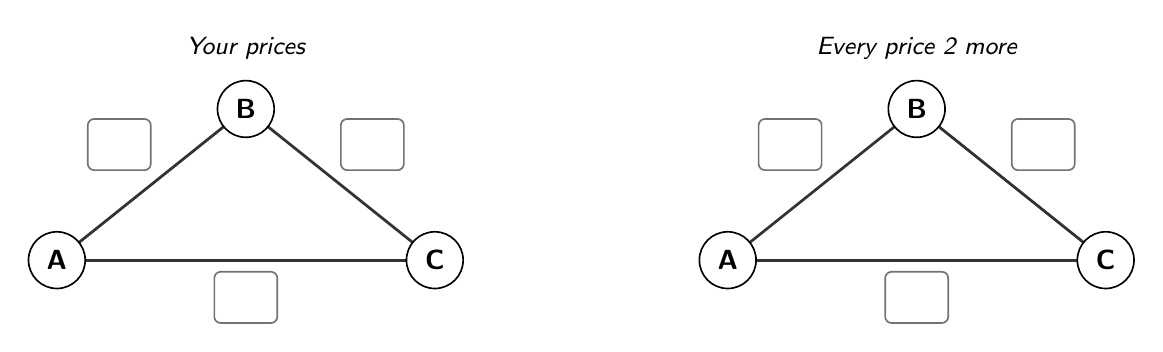
\begin{tikzpicture}[x=1mm,y=1mm]
\draw[line width=1.0pt, black!80] (3.60,7.98) -- (27.60,27.18);
\draw[line width=1.0pt, black!80] (27.60,27.18) -- (51.60,7.98);
\draw[line width=1.0pt, black!80] (3.60,7.98) -- (51.60,7.98);
\draw[black!55, line width=0.6pt, fill=white, rounded corners=0.8mm] (7.53,19.41) rectangle (15.53,25.91);
\draw[black!55, line width=0.6pt, fill=white, rounded corners=0.8mm] (39.67,19.41) rectangle (47.67,25.91);
\draw[black!55, line width=0.6pt, fill=white, rounded corners=0.8mm] (23.60,0.00) rectangle (31.60,6.50);
\node[circle, draw, line width=0.6pt, fill=white, minimum size=7.20mm, inner sep=0, font=\normalsize\bfseries] at (3.60,7.98) {A};
\node[circle, draw, line width=0.6pt, fill=white, minimum size=7.20mm, inner sep=0, font=\normalsize\bfseries] at (27.60,27.18) {B};
\node[circle, draw, line width=0.6pt, fill=white, minimum size=7.20mm, inner sep=0, font=\normalsize\bfseries] at (51.60,7.98) {C};
\node[font=\small\itshape, anchor=south, align=center] at (27.60,32.28) {Your prices};
\draw[line width=1.0pt, black!80] (88.80,7.98) -- (112.80,27.18);
\draw[line width=1.0pt, black!80] (112.80,27.18) -- (136.80,7.98);
\draw[line width=1.0pt, black!80] (88.80,7.98) -- (136.80,7.98);
\draw[black!55, line width=0.6pt, fill=white, rounded corners=0.8mm] (92.73,19.41) rectangle (100.73,25.91);
\draw[black!55, line width=0.6pt, fill=white, rounded corners=0.8mm] (124.87,19.41) rectangle (132.87,25.91);
\draw[black!55, line width=0.6pt, fill=white, rounded corners=0.8mm] (108.80,0.00) rectangle (116.80,6.50);
\node[circle, draw, line width=0.6pt, fill=white, minimum size=7.20mm, inner sep=0, font=\normalsize\bfseries] at (88.80,7.98) {A};
\node[circle, draw, line width=0.6pt, fill=white, minimum size=7.20mm, inner sep=0, font=\normalsize\bfseries] at (112.80,27.18) {B};
\node[circle, draw, line width=0.6pt, fill=white, minimum size=7.20mm, inner sep=0, font=\normalsize\bfseries] at (136.80,7.98) {C};
\node[font=\small\itshape, anchor=south, align=center] at (112.80,32.28) {Every price 2 more};
\end{tikzpicture}
\end{center}\par

\vspace{-2mm}
\par\begin{center}
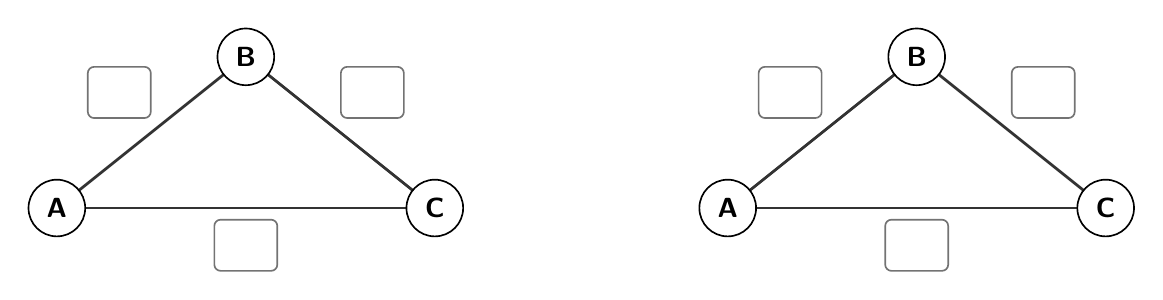
\begin{tikzpicture}[x=1mm,y=1mm]
\draw[line width=1.0pt, black!80] (3.60,7.98) -- (27.60,27.18);
\draw[line width=1.0pt, black!80] (27.60,27.18) -- (51.60,7.98);
\draw[line width=1.0pt, black!80] (3.60,7.98) -- (51.60,7.98);
\draw[black!55, line width=0.6pt, fill=white, rounded corners=0.8mm] (7.53,19.41) rectangle (15.53,25.91);
\draw[black!55, line width=0.6pt, fill=white, rounded corners=0.8mm] (39.67,19.41) rectangle (47.67,25.91);
\draw[black!55, line width=0.6pt, fill=white, rounded corners=0.8mm] (23.60,0.00) rectangle (31.60,6.50);
\node[circle, draw, line width=0.6pt, fill=white, minimum size=7.20mm, inner sep=0, font=\normalsize\bfseries] at (3.60,7.98) {A};
\node[circle, draw, line width=0.6pt, fill=white, minimum size=7.20mm, inner sep=0, font=\normalsize\bfseries] at (27.60,27.18) {B};
\node[circle, draw, line width=0.6pt, fill=white, minimum size=7.20mm, inner sep=0, font=\normalsize\bfseries] at (51.60,7.98) {C};
\draw[line width=1.0pt, black!80] (88.80,7.98) -- (112.80,27.18);
\draw[line width=1.0pt, black!80] (112.80,27.18) -- (136.80,7.98);
\draw[line width=1.0pt, black!80] (88.80,7.98) -- (136.80,7.98);
\draw[black!55, line width=0.6pt, fill=white, rounded corners=0.8mm] (92.73,19.41) rectangle (100.73,25.91);
\draw[black!55, line width=0.6pt, fill=white, rounded corners=0.8mm] (124.87,19.41) rectangle (132.87,25.91);
\draw[black!55, line width=0.6pt, fill=white, rounded corners=0.8mm] (108.80,0.00) rectangle (116.80,6.50);
\node[circle, draw, line width=0.6pt, fill=white, minimum size=7.20mm, inner sep=0, font=\normalsize\bfseries] at (88.80,7.98) {A};
\node[circle, draw, line width=0.6pt, fill=white, minimum size=7.20mm, inner sep=0, font=\normalsize\bfseries] at (112.80,27.18) {B};
\node[circle, draw, line width=0.6pt, fill=white, minimum size=7.20mm, inner sep=0, font=\normalsize\bfseries] at (136.80,7.98) {C};
\end{tikzpicture}
\end{center}\par

\vspace{-2mm}
\par\begin{center}
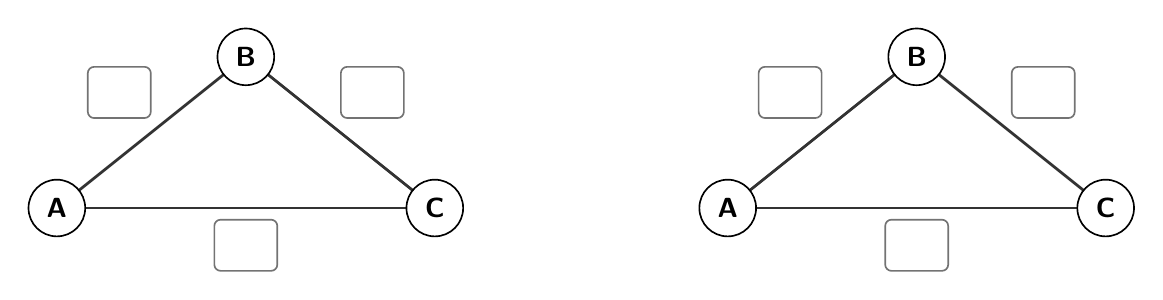
\begin{tikzpicture}[x=1mm,y=1mm]
\draw[line width=1.0pt, black!80] (3.60,7.98) -- (27.60,27.18);
\draw[line width=1.0pt, black!80] (27.60,27.18) -- (51.60,7.98);
\draw[line width=1.0pt, black!80] (3.60,7.98) -- (51.60,7.98);
\draw[black!55, line width=0.6pt, fill=white, rounded corners=0.8mm] (7.53,19.41) rectangle (15.53,25.91);
\draw[black!55, line width=0.6pt, fill=white, rounded corners=0.8mm] (39.67,19.41) rectangle (47.67,25.91);
\draw[black!55, line width=0.6pt, fill=white, rounded corners=0.8mm] (23.60,0.00) rectangle (31.60,6.50);
\node[circle, draw, line width=0.6pt, fill=white, minimum size=7.20mm, inner sep=0, font=\normalsize\bfseries] at (3.60,7.98) {A};
\node[circle, draw, line width=0.6pt, fill=white, minimum size=7.20mm, inner sep=0, font=\normalsize\bfseries] at (27.60,27.18) {B};
\node[circle, draw, line width=0.6pt, fill=white, minimum size=7.20mm, inner sep=0, font=\normalsize\bfseries] at (51.60,7.98) {C};
\draw[line width=1.0pt, black!80] (88.80,7.98) -- (112.80,27.18);
\draw[line width=1.0pt, black!80] (112.80,27.18) -- (136.80,7.98);
\draw[line width=1.0pt, black!80] (88.80,7.98) -- (136.80,7.98);
\draw[black!55, line width=0.6pt, fill=white, rounded corners=0.8mm] (92.73,19.41) rectangle (100.73,25.91);
\draw[black!55, line width=0.6pt, fill=white, rounded corners=0.8mm] (124.87,19.41) rectangle (132.87,25.91);
\draw[black!55, line width=0.6pt, fill=white, rounded corners=0.8mm] (108.80,0.00) rectangle (116.80,6.50);
\node[circle, draw, line width=0.6pt, fill=white, minimum size=7.20mm, inner sep=0, font=\normalsize\bfseries] at (88.80,7.98) {A};
\node[circle, draw, line width=0.6pt, fill=white, minimum size=7.20mm, inner sep=0, font=\normalsize\bfseries] at (112.80,27.18) {B};
\node[circle, draw, line width=0.6pt, fill=white, minimum size=7.20mm, inner sep=0, font=\normalsize\bfseries] at (136.80,7.98) {C};
\end{tikzpicture}
\end{center}\par

\vspace{-2mm}
\vspace{6mm}
\prob{7} Can adding the same number to every price of a map ever change which networks are cheapest? Can doubling every price ever change the cheapest trips? Explain.
\newpage

\prob{8} On these maps, a network must join the circled places, and it may go through the place in a square or leave it out. On each map, find the cheapest network, once without the square and once using it.

\par\begin{center}
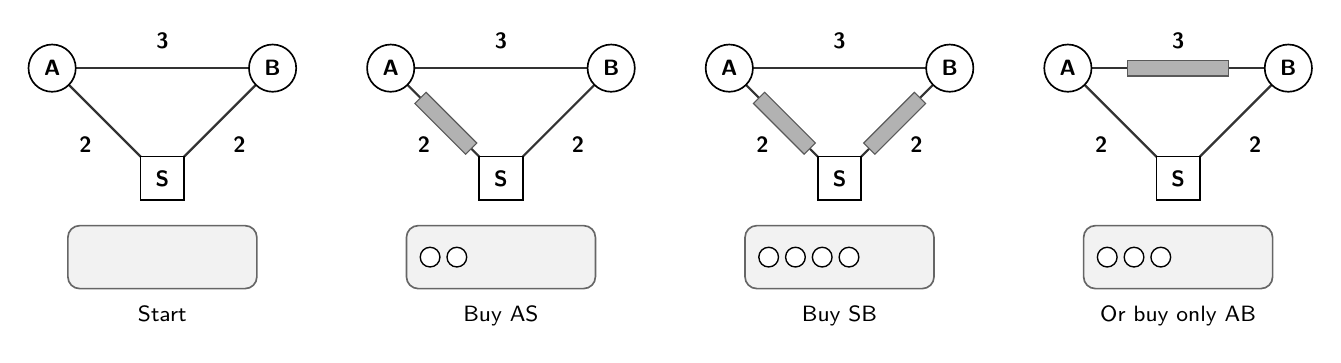
\begin{tikzpicture}[x=1mm,y=1mm]
\draw[line width=0.8pt, black!80] (3.00,29.00) -- (31.00,29.00);
\draw[line width=0.8pt, black!80] (3.00,29.00) -- (17.00,15.00);
\draw[line width=0.8pt, black!80] (17.00,15.00) -- (31.00,29.00);
\node[fill=white, inner sep=0, minimum width=2.80mm, minimum height=3.40mm, font=\footnotesize\bfseries] at (17.00,32.44) {3};
\node[fill=white, inner sep=0, minimum width=2.80mm, minimum height=3.40mm, font=\footnotesize\bfseries] at (7.22,19.22) {2};
\node[fill=white, inner sep=0, minimum width=2.80mm, minimum height=3.40mm, font=\footnotesize\bfseries] at (26.78,19.22) {2};
\node[circle, draw, line width=0.6pt, fill=white, minimum size=6.00mm, inner sep=0, font=\footnotesize\bfseries] at (3.00,29.00) {A};
\node[circle, draw, line width=0.6pt, fill=white, minimum size=6.00mm, inner sep=0, font=\footnotesize\bfseries] at (31.00,29.00) {B};
\node[rectangle, draw, line width=0.6pt, fill=white, minimum size=5.52mm, inner sep=0, font=\footnotesize\bfseries] at (17.00,15.00) {S};
\draw[black!60, line width=0.6pt, fill=black!5, rounded corners=1.5mm] (5.00,1.00) rectangle (29.00,9.00);
\node[font=\footnotesize, anchor=north, align=center] at (17.00,0.00) {Start};
\draw[line width=0.8pt, black!80] (46.00,29.00) -- (74.00,29.00);
\draw[line width=0.8pt, black!80] (46.00,29.00) -- (60.00,15.00);
\draw[line width=0.8pt, black!80] (60.00,15.00) -- (74.00,29.00);
\filldraw[fill=black!30, draw=black!65, line width=0.4pt] (50.49,25.93) -- (56.93,19.49) -- (55.51,18.07) -- (49.07,24.51) -- cycle;
\node[fill=white, inner sep=0, minimum width=2.80mm, minimum height=3.40mm, font=\footnotesize\bfseries] at (60.00,32.44) {3};
\node[fill=white, inner sep=0, minimum width=2.80mm, minimum height=3.40mm, font=\footnotesize\bfseries] at (50.22,19.22) {2};
\node[fill=white, inner sep=0, minimum width=2.80mm, minimum height=3.40mm, font=\footnotesize\bfseries] at (69.78,19.22) {2};
\node[circle, draw, line width=0.6pt, fill=white, minimum size=6.00mm, inner sep=0, font=\footnotesize\bfseries] at (46.00,29.00) {A};
\node[circle, draw, line width=0.6pt, fill=white, minimum size=6.00mm, inner sep=0, font=\footnotesize\bfseries] at (74.00,29.00) {B};
\node[rectangle, draw, line width=0.6pt, fill=white, minimum size=5.52mm, inner sep=0, font=\footnotesize\bfseries] at (60.00,15.00) {S};
\draw[black!60, line width=0.6pt, fill=black!5, rounded corners=1.5mm] (48.00,1.00) rectangle (72.00,9.00);
\draw[line width=0.5pt, fill=white] (51.00,5.00) circle (1.25mm);
\draw[line width=0.5pt, fill=white] (54.40,5.00) circle (1.25mm);
\node[font=\footnotesize, anchor=north, align=center] at (60.00,0.00) {Buy AS};
\draw[line width=0.8pt, black!80] (89.00,29.00) -- (117.00,29.00);
\draw[line width=0.8pt, black!80] (89.00,29.00) -- (103.00,15.00);
\draw[line width=0.8pt, black!80] (103.00,15.00) -- (117.00,29.00);
\filldraw[fill=black!30, draw=black!65, line width=0.4pt] (93.49,25.93) -- (99.93,19.49) -- (98.51,18.07) -- (92.07,24.51) -- cycle;
\filldraw[fill=black!30, draw=black!65, line width=0.4pt] (106.07,19.49) -- (112.51,25.93) -- (113.93,24.51) -- (107.49,18.07) -- cycle;
\node[fill=white, inner sep=0, minimum width=2.80mm, minimum height=3.40mm, font=\footnotesize\bfseries] at (103.00,32.44) {3};
\node[fill=white, inner sep=0, minimum width=2.80mm, minimum height=3.40mm, font=\footnotesize\bfseries] at (93.22,19.22) {2};
\node[fill=white, inner sep=0, minimum width=2.80mm, minimum height=3.40mm, font=\footnotesize\bfseries] at (112.78,19.22) {2};
\node[circle, draw, line width=0.6pt, fill=white, minimum size=6.00mm, inner sep=0, font=\footnotesize\bfseries] at (89.00,29.00) {A};
\node[circle, draw, line width=0.6pt, fill=white, minimum size=6.00mm, inner sep=0, font=\footnotesize\bfseries] at (117.00,29.00) {B};
\node[rectangle, draw, line width=0.6pt, fill=white, minimum size=5.52mm, inner sep=0, font=\footnotesize\bfseries] at (103.00,15.00) {S};
\draw[black!60, line width=0.6pt, fill=black!5, rounded corners=1.5mm] (91.00,1.00) rectangle (115.00,9.00);
\draw[line width=0.5pt, fill=white] (94.00,5.00) circle (1.25mm);
\draw[line width=0.5pt, fill=white] (97.40,5.00) circle (1.25mm);
\draw[line width=0.5pt, fill=white] (100.80,5.00) circle (1.25mm);
\draw[line width=0.5pt, fill=white] (104.20,5.00) circle (1.25mm);
\node[font=\footnotesize, anchor=north, align=center] at (103.00,0.00) {Buy SB};
\draw[line width=0.8pt, black!80] (132.00,29.00) -- (160.00,29.00);
\draw[line width=0.8pt, black!80] (132.00,29.00) -- (146.00,15.00);
\draw[line width=0.8pt, black!80] (146.00,15.00) -- (160.00,29.00);
\filldraw[fill=black!30, draw=black!65, line width=0.4pt] (139.56,30.00) -- (152.44,30.00) -- (152.44,28.00) -- (139.56,28.00) -- cycle;
\node[fill=white, inner sep=0, minimum width=2.80mm, minimum height=3.40mm, font=\footnotesize\bfseries] at (146.00,32.44) {3};
\node[fill=white, inner sep=0, minimum width=2.80mm, minimum height=3.40mm, font=\footnotesize\bfseries] at (136.22,19.22) {2};
\node[fill=white, inner sep=0, minimum width=2.80mm, minimum height=3.40mm, font=\footnotesize\bfseries] at (155.78,19.22) {2};
\node[circle, draw, line width=0.6pt, fill=white, minimum size=6.00mm, inner sep=0, font=\footnotesize\bfseries] at (132.00,29.00) {A};
\node[circle, draw, line width=0.6pt, fill=white, minimum size=6.00mm, inner sep=0, font=\footnotesize\bfseries] at (160.00,29.00) {B};
\node[rectangle, draw, line width=0.6pt, fill=white, minimum size=5.52mm, inner sep=0, font=\footnotesize\bfseries] at (146.00,15.00) {S};
\draw[black!60, line width=0.6pt, fill=black!5, rounded corners=1.5mm] (134.00,1.00) rectangle (158.00,9.00);
\draw[line width=0.5pt, fill=white] (137.00,5.00) circle (1.25mm);
\draw[line width=0.5pt, fill=white] (140.40,5.00) circle (1.25mm);
\draw[line width=0.5pt, fill=white] (143.80,5.00) circle (1.25mm);
\node[font=\footnotesize, anchor=north, align=center] at (146.00,0.00) {Or buy only AB};
\end{tikzpicture}
\end{center}\par

\vspace{1mm}
\par\begin{center}
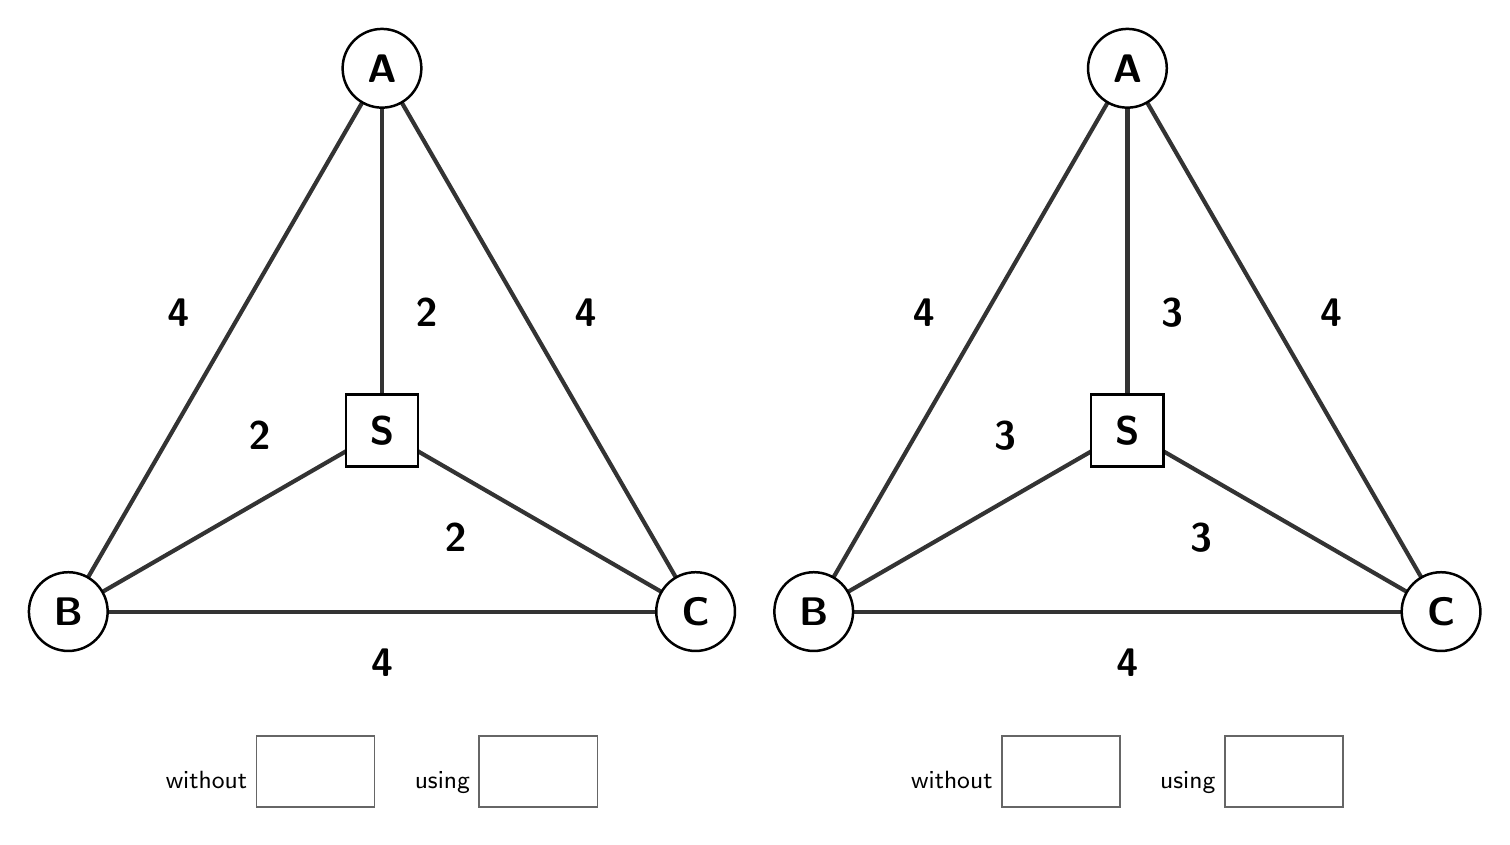
\begin{tikzpicture}[x=1mm,y=1mm]
\draw[line width=1.5pt, black!80] (44.84,92.46) -- (5.00,23.46);
\draw[line width=1.5pt, black!80] (5.00,23.46) -- (84.67,23.46);
\draw[line width=1.5pt, black!80] (44.84,92.46) -- (84.67,23.46);
\draw[line width=1.5pt, black!80] (44.84,46.46) -- (44.84,92.46);
\draw[line width=1.5pt, black!80] (44.84,46.46) -- (5.00,23.46);
\draw[line width=1.5pt, black!80] (44.84,46.46) -- (84.67,23.46);
\node[fill=white, inner sep=0, minimum width=4.40mm, minimum height=6.00mm, font=\Large\bfseries] at (18.97,61.40) {4};
\node[fill=white, inner sep=0, minimum width=4.40mm, minimum height=6.00mm, font=\Large\bfseries] at (44.84,17.00) {4};
\node[fill=white, inner sep=0, minimum width=4.40mm, minimum height=6.00mm, font=\Large\bfseries] at (70.70,61.40) {4};
\node[fill=white, inner sep=0, minimum width=4.40mm, minimum height=6.00mm, font=\Large\bfseries] at (50.50,61.41) {2};
\node[fill=white, inner sep=0, minimum width=4.40mm, minimum height=6.00mm, font=\Large\bfseries] at (29.30,45.77) {2};
\node[fill=white, inner sep=0, minimum width=4.40mm, minimum height=6.00mm, font=\Large\bfseries] at (54.20,32.79) {2};
\node[circle, draw, line width=0.9pt, fill=white, minimum size=10.00mm, inner sep=0, font=\Large\bfseries] at (44.84,92.46) {A};
\node[circle, draw, line width=0.9pt, fill=white, minimum size=10.00mm, inner sep=0, font=\Large\bfseries] at (5.00,23.46) {B};
\node[circle, draw, line width=0.9pt, fill=white, minimum size=10.00mm, inner sep=0, font=\Large\bfseries] at (84.67,23.46) {C};
\node[rectangle, draw, line width=0.9pt, fill=white, minimum size=9.20mm, inner sep=0, font=\Large\bfseries] at (44.84,46.46) {S};
\node[anchor=north, font=\small] at (44.84,9) {without \raisebox{-2.5mm}{\tikz[x=1mm,y=1mm]{\draw[black!60, line width=0.6pt] (0,0) rectangle (15,9);}}\hspace{5mm}using \raisebox{-2.5mm}{\tikz[x=1mm,y=1mm]{\draw[black!60, line width=0.6pt] (0,0) rectangle (15,9);}}};
\draw[line width=1.5pt, black!80] (139.51,92.46) -- (99.67,23.46);
\draw[line width=1.5pt, black!80] (99.67,23.46) -- (179.34,23.46);
\draw[line width=1.5pt, black!80] (139.51,92.46) -- (179.34,23.46);
\draw[line width=1.5pt, black!80] (139.51,46.46) -- (139.51,92.46);
\draw[line width=1.5pt, black!80] (139.51,46.46) -- (99.67,23.46);
\draw[line width=1.5pt, black!80] (139.51,46.46) -- (179.34,23.46);
\node[fill=white, inner sep=0, minimum width=4.40mm, minimum height=6.00mm, font=\Large\bfseries] at (113.64,61.40) {4};
\node[fill=white, inner sep=0, minimum width=4.40mm, minimum height=6.00mm, font=\Large\bfseries] at (139.51,17.00) {4};
\node[fill=white, inner sep=0, minimum width=4.40mm, minimum height=6.00mm, font=\Large\bfseries] at (165.38,61.40) {4};
\node[fill=white, inner sep=0, minimum width=4.40mm, minimum height=6.00mm, font=\Large\bfseries] at (145.17,61.41) {3};
\node[fill=white, inner sep=0, minimum width=4.40mm, minimum height=6.00mm, font=\Large\bfseries] at (123.98,45.77) {3};
\node[fill=white, inner sep=0, minimum width=4.40mm, minimum height=6.00mm, font=\Large\bfseries] at (148.87,32.79) {3};
\node[circle, draw, line width=0.9pt, fill=white, minimum size=10.00mm, inner sep=0, font=\Large\bfseries] at (139.51,92.46) {A};
\node[circle, draw, line width=0.9pt, fill=white, minimum size=10.00mm, inner sep=0, font=\Large\bfseries] at (99.67,23.46) {B};
\node[circle, draw, line width=0.9pt, fill=white, minimum size=10.00mm, inner sep=0, font=\Large\bfseries] at (179.34,23.46) {C};
\node[rectangle, draw, line width=0.9pt, fill=white, minimum size=9.20mm, inner sep=0, font=\Large\bfseries] at (139.51,46.46) {S};
\node[anchor=north, font=\small] at (139.51,9) {without \raisebox{-2.5mm}{\tikz[x=1mm,y=1mm]{\draw[black!60, line width=0.6pt] (0,0) rectangle (15,9);}}\hspace{5mm}using \raisebox{-2.5mm}{\tikz[x=1mm,y=1mm]{\draw[black!60, line width=0.6pt] (0,0) rectangle (15,9);}}};
\end{tikzpicture}
\end{center}\par

\vspace{1mm}
\end{document}
